%%%%%%%%%%%%%%%%%%%%%%%%%%%%%%%%%%%%%%%%%
% Classicthesis Typographic Thesis
% LaTeX Template
% Version 1.4 (1/1/16)
%
% This template has been downloaded from:
% http://www.LaTeXTemplates.com
%
% Original author:
% André Miede (http://www.miede.de) with commenting modifications by:
% Vel (vel@LaTeXTemplates.com)
%
% License:
% GNU General Public License (v2)
%
% General Tips:
% 1) Make sure to edit the classicthesis-config.file
% 2) New enumeration (A., B., C., etc in small caps): \begin{aenumerate} \end{aenumerate}
% 3) For margin notes: \marginpar or \graffito{}
% 4) Do not use bold fonts in this style, it is designed around them
% 5) Use tables as in the examples
% 6) See classicthesis-preamble.sty for useful commands
%
%%%%%%%%%%%%%%%%%%%%%%%%%%%%%%%%%%%%%%%%%

%----------------------------------------------------------------------------------------
%	PACKAGES AND OTHER DOCUMENT CONFIGURATIONS
%----------------------------------------------------------------------------------------
\documentclass[
  % double side thesis
  twoside,openright,
  % primary font size
  fontsize=10pt,
  paper=b5,
  % new page after the title
  titlepage,
  % no point after section number
  dottedtoc,
  % header and footer at foot of the page
  headinclude=true,
  footinclude=true,
  % 5 mm bookbinding
  BCOR=5mm,
  % empty pages without header at foot of the page
  cleardoublepage=empty,
  abstract=on,
  parskip=half,
  DIV=calc,
  % Languages
  american
]{scrreprt}


% Includes the file which contains all the document configurations and packages - make sure to edit this file
%%%%%%%%%%%%%%%%%%%%%%%%%%%%%%%%%%%%%%%%%
% Classicthesis Typographic Thesis
% Configuration File
%
% This file has been downloaded from:
% http://www.LaTeXTemplates.com
%
% Original author:
% André Miede (http://www.miede.de) with extensive commenting changes by:
% Vel (vel@LaTeXTemplates.com)
%
% License:
% GNU General Public License (v2)
%
% Important note:
% The main lines to change in this file are in the DOCUMENT VARIABLES
% section, the rest of the file is for advanced configuration.
%
%%%%%%%%%%%%%%%%%%%%%%%%%%%%%%%%%%%%%%%%%

%----------------------------------------------------------------------------------------
%	CHARACTER ENCODING
%----------------------------------------------------------------------------------------

\PassOptionsToPackage{utf8}{inputenc} % Set the encoding of your files. UTF-8 is the only sensible encoding nowadays. If you can't read äöüßáéçèê∂åëæƒÏ€ then change the encoding setting in your editor, not the line below. If your editor does not support utf8 use another editor!
\usepackage{inputenc}

%----------------------------------------------------------------------------------------
%	DOCUMENT VARIABLES
%	Fill in the lines below to enter your information into the thesis template
%	Each of the commands can be cited anywhere in the thesis
%----------------------------------------------------------------------------------------

% Remove drafting to get rid of the '[ Date - classicthesis version 4.0 ]' text at the bottom of every page
\PassOptionsToPackage{
  % print version information on the bottom of the pages
  drafting=false,
  % the left column of the toc will be aligned (no indentation)
  tocaligned=false,
  % page numbers in ToC flushed right
  dottedtoc=false,
  % use AMS Euler for chapter font (otherwise Palatino)
  eulerchapternumbers=true,
  % chaper headers will have line above and beneath
  linedheaders=false,
  % numbering per chapter for all floats (i.e., Figure 1.1)
  floatperchapter=true,
  % use awesome Euler fonts for mathematical formulae (only with pdfLaTeX)
  eulermath=false,
  % toggle a nice monospaced font (w/ bold)
  beramono=true,
  % deactivate standard font for loading another one, see the last section at the end of this file for suggestions
  palatino=true,
  style= classicthesis%, arsclassica
}{classicthesis}

%\PassOptionsToPackage{eulerchapternumbers,listings,drafting, pdfspacing, subfig,beramono,eulermath,parts, style = classicthesis-arsclassica}
%{classicthesis}
% Available options: drafting parts nochapters linedheaders eulerchapternumbers beramono eulermath pdfspacing minionprospacing tocaligned dottedtoc manychapters listings floatperchapter subfig

%\usepackage{scrpage}

%\deftripstyle{pgnumbottomcenter}{}{}{}{}{\pagemark{}}{}
%\pagestyle{pgnumbottomcenter}
%\renewcommand{\chapterpagestyle}{pgnumbottomcenter}
% Understanding the emergence con context dependent interactions in
\newcommand{\myTitle}{Increasing realism in models of biotic interactions:\xspace}
\newcommand{\mySubtitle}{ecological and evolutionary consequences }
\newcommand{\myDegree}{Doctoral thesis\xspace}
\newcommand{\myName}{Alba Cervantes Loreto\xspace}
\newcommand{\myProf}{Daniel B. Stouffer\xspace}
%\newcommand{\mySupervisor}{Daniel B. Stouffer\xspace}
\newcommand{\myFaculty}{College of Science\xspace}
\newcommand{\myDepartment}{School of Biological Sciences\xspace}
\newcommand{\myUni}{University of Canterbury\xspace}
\newcommand{\myLocation}{Christchurch, New Zealand\xspace}
\newcommand{\myTime}{November 2021\xspace}
\newcommand{\myVersion}{Version 1.0}
%Disentangling the emergence and consequences of context dependent interactions in ecological and evolutionary dynamics
%------------------------------------------------------------------------------
% Setup, finetuning, and useful commands
%------------------------------------------------------------------------------

\providecommand{\mLyX}{L\kern-.1667em\lower.25em\hbox{Y}\kern-.125emX\@}
\newcommand{\ie}{i.\,e.}
\newcommand{\Ie}{I.\,e.}
\newcommand{\eg}{e.\,g.}
\newcommand{\Eg}{E.\,g.}

%----------------------------------------------------------------------------------------
%	PACKAGES
%----------------------------------------------------------------------------------------

\usepackage[unicode=true, pdfpagelabels]{hyperref}
\usepackage{float}
\usepackage[font=footnotesize]{caption}
\usepackage{pdflscape}
\usepackage[pdftex]{graphicx}
\usepackage{adforn}

\usepackage{url}
\usepackage{longtable}
\usepackage{setspace}
\doublespacing
\usepackage{rotating}
\usepackage{lineno}
\usepackage{mdframed} % to create frame around text
\usepackage{rotating} % to rotate table
\usepackage{tabularx}


%------------------------------------------------

%\PassOptionsToPackage{ngerman,american}{babel}  % Change this to your language(s)
\PassOptionsToPackage{main=british}{babel}
\usepackage{babel}

%------------------------------------------------

\usepackage{csquotes}
\PassOptionsToPackage{%
%backend=biber, % Instead of bibtex
backend=bibtex8,bibencoding=ascii,%
language=auto,%
%style=numeric-comp,%
style=authoryear-comp, % Author 1999, 2010
%bibstyle=authoryear,dashed=false, % dashed: substitute rep. author with ---
sorting=nyt, % name, year, title
maxbibnames=10, % default: 3, et al.
%backref=true,%
natbib=true % natbib compatibility mode (\citep and \citet still work)
}{biblatex}
\usepackage{biblatex}

 %------------------------------------------------

\PassOptionsToPackage{fleqn}{amsmath} % Math environments and more by the AMS
 \usepackage{amsmath}

 %------------------------------------------------

\PassOptionsToPackage{T1}{fontenc} % T2A for cyrillics
\usepackage{fontenc}

%------------------------------------------------

\usepackage{textcomp} % Fix warning with missing font shapes

%------------------------------------------------

\usepackage{scrhack} % Fix warnings when using KOMA with listings package

%------------------------------------------------

\usepackage{xspace} % To get the spacing after macros right

%------------------------------------------------

\usepackage{mparhack} % To get marginpar right

%------------------------------------------------

\usepackage{fixltx2e} % Fixes some LaTeX stuff

%------------------------------------------------

\PassOptionsToPackage{smaller}{acronym} % Include printonlyused in the first bracket to only show acronyms used in the text
\usepackage{acronym} % Nice macros for handling all acronyms in the thesis

%\renewcommand*{\acsfont}[1]{\textssc{#1}} % For MinionPro
\renewcommand*{\aclabelfont}[1]{\acsfont{#1}}

%------------------------------------------------

\PassOptionsToPackage{pdftex}{graphicx}
\usepackage{graphicx}

%----------------------------------------------------------------------------------------
%	FLOATS: TABLES, FIGURES AND CAPTIONS SETUP
%----------------------------------------------------------------------------------------
\usepackage[strict]{changepage}
\usepackage{booktabs,tabularx} % Better tables
\usepackage{multirow} % multirow/ multicol tables
\setlength{\extrarowheight}{3pt} % Increase table row height
\newcommand{\tableheadline}[1]{\multicolumn{1}{c}{\spacedlowsmallcaps{#1}}}
\newcommand{\myfloatalign}{\centering} % To be used with each float for alignment
\usepackage{caption}
\captionsetup{font=small}
\usepackage{subfig}
% SO that floats that are larger than this number get their own page
\renewcommand{\floatpagefraction}{.4}

%----------------------------------------------------------------------------------------
%	HYPERREFERENCES
%----------------------------------------------------------------------------------------

\PassOptionsToPackage{pdftex,hyperfootnotes=false,pdfpagelabels}{hyperref}
\usepackage{hyperref}  % backref linktocpage pagebackref
\pdfcompresslevel=9
\pdfadjustspacing=1

\hypersetup{
% Uncomment the line below to remove all links (to references, figures, tables, etc), useful for b/w printouts
%draft,
colorlinks=true, linktocpage=true, pdfstartpage=3, pdfstartview=FitV,
% Uncomment the line below if you want to have black links (e.g. for printing black and white)
%colorlinks=false, linktocpage=false, pdfborder={0 0 0}, pdfstartpage=3, pdfstartview=FitV,
breaklinks=true, pdfpagemode=UseNone, pageanchor=true, pdfpagemode=UseOutlines,%
plainpages=false, bookmarksnumbered, bookmarksopen=true, bookmarksopenlevel=1,%
hypertexnames=true, pdfhighlight=/O,%nesting=true,%frenchlinks,%
urlcolor=Maroon, linkcolor=Maroon, citecolor=Maroon, pagecolor=Maroon, %pagecolor=RoyalBlue,%
    %urlcolor=Black, linkcolor=Black, citecolor=Black, %pagecolor=Black,%
%------------------------------------------------
% PDF file meta-information
pdftitle={\myTitle},
pdfauthor={\textcopyright\ \myName, \myUni, \myFaculty},
pdfsubject={},
pdfkeywords={},
pdfcreator={pdfLaTeX},
pdfproducer={LaTeX with hyperref and classicthesis}
%------------------------------------------------
}

%----------------------------------------------------------------------------------------
%	AUTOREFERENCES SETUP
%	Redefines how references in text are prefaced for different
%	languages (e.g. "Section 1.2" or "section 1.2")
%----------------------------------------------------------------------------------------

\makeatletter
\@ifpackageloaded{babel}
{
\addto\extrasamerican{
\renewcommand*{\figureautorefname}{Figure}
\renewcommand*{\tableautorefname}{Table}
\renewcommand*{\partautorefname}{Part}
\renewcommand*{\chapterautorefname}{Chapter}
\renewcommand*{\sectionautorefname}{Section}
\renewcommand*{\subsectionautorefname}{Section}
\renewcommand*{\subsubsectionautorefname}{Section}
}
\addto\extrasngerman{
\renewcommand*{\paragraphautorefname}{Absatz}
\renewcommand*{\subparagraphautorefname}{Unterabsatz}
\renewcommand*{\footnoteautorefname}{Fu\"snote}
\renewcommand*{\FancyVerbLineautorefname}{Zeile}
\renewcommand*{\theoremautorefname}{Theorem}
\renewcommand*{\appendixautorefname}{Anhang}
\renewcommand*{\equationautorefname}{Gleichung}
\renewcommand*{\itemautorefname}{Punkt}
}
\providecommand{\subfigureautorefname}{\figureautorefname} % Fix to getting autorefs for subfigures right
}{\relax}
\makeatother

%----------------------------------------------------------------------------------------
\usepackage{classicthesis}

% Remove useless warnings
\RequirePackage{silence} % :-\
    \WarningFilter{scrreprt}{Usage of package `titlesec'}
    \WarningFilter{scrreprt}{Activating an ugly workaround}
    \WarningFilter{titlesec}{Non standard sectioning command detected}

\clearscrheadfoot
\ohead[]{\headmark}
\rofoot[\pagemark]{\pagemark}
\lefoot[\pagemark]{\pagemark}

\addbibresource{Bibliography} % The file housing your bibliography
%\addbibresource[label=ownpubs]{Self_Publications.bib} % Uncomment for optional self-publications

%\hyphenation{Put special hyphenation here}

\begin{document}

\frenchspacing % Reduces space after periods to make text more compact

\raggedbottom % Makes all pages the height of the text on that page

\selectlanguage{american} % Select your default language - e.g. american or ngerman


\pagenumbering{roman} % Roman page numbering prior to the start of the thesis content (i, ii, iii, etc)
\setcounter{page}{1}
\pagestyle{plain} % Suppress headers for the pre-content pages

%----------------------------------------------------------------------------------------
%	PRE-CONTENT THESIS PAGES
%----------------------------------------------------------------------------------------

\begin{titlepage}
    %\pdfbookmark[1]{\myTitle}{titlepage}
    % if you want the titlepage to be centered, uncomment and fine-tune the line below (KOMA classes environment)
    \begin{addmargin}[-1cm]{-3cm}
    \begin{center}
        \large

        \hfill
        \vfill

        \begingroup
        \huge
        \color{webbrown}\spacedallcaps{\myTitle} \\ \bigskip
        \endgroup

        \begingroup
          \Large
          \textit{\mySubtitle}
        \endgroup


        \bigskip
        \bigskip
        \bigskip

        \begingroup
        \huge
        \adforn{21}
        \endgroup

        \bigskip
        \bigskip
        \bigskip

        \begingroup
        \Large
        \spacedlowsmallcaps{\myName} \\ \medskip
        \endgroup
        %\myTime\ -- \myVersion

        \bigskip
        \bigskip
        \bigskip
        \bigskip
        \bigskip
        
        \vfill
        \large \textit{A thesis submitted in fulfillment of the requirements\\ for the degree of Doctor of Philosophy}\\[0.3cm] % University requirement text

        
        
         \bigskip
        \bigskip
        \bigskip
        \bigskip
        \bigskip
        
        \begingroup
        \normalsize
        \myDepartment \\
         \myFaculty \\
        \myUni \\
        \endgroup


        \vfill

    \end{center}
  \end{addmargin}
\end{titlepage} % Main title page

% Back of the title page

\thispagestyle{empty}

\hfill

\vfill

\noindent\myName. \textit{\myTitle} \mySubtitle; \myDegree, \myTime

\bigskip
%
\noindent\spacedlowsmallcaps{Supervisor}: \\
\myProf
 %\\
% \mySupervisor
%
\medskip

\noindent\spacedlowsmallcaps{Co-supervisors}: \\
Margaret M. Mayfield \\
Andrew Letten
%Janneke Hille Ris Lambers\\
%to be determined
% \mySupervisor
%
\medskip

%\noindent\spacedlowsmallcaps{Location}: \\
\noindent\myLocation

%\medskip

%\noindent\spacedlowsmallcaps{Date}: \\
%\myTime
 % Back of the title page

\cleardoublepage% Dedication

\thispagestyle{empty}
\pdfbookmark[1]{Dedication}{Dedication} % Bookmark name visible in a PDF viewer

\vspace*{3cm}

\begin{center}
\flushleft
Different abstractions from the same wholes capture different aspects of the reality but also leave us with different blindnesses. Therefore it is always necessary to recognize that our abstractions are intellectual constructs, that an ‘‘object’’ kicks and screams when it is abstracted from its context and may take its revenge in leading us astray.

	\flushright -- Richard Levins 
\end{center}

\medskip
 % Dedication page

%\cleardoublepage\include{FrontBackMatter/Foreword} % Uncomment and create a Foreword.tex to include a foreword

\cleardoublepage\pdfbookmark[1]{Abstract}{Abstract} % Bookmark name visible in a PDF viewer
\chapter*{Abstract}
\small
Interactions between organisms have a central role in the study of ecological and evolutionary dynamics. The study of biotic interactions usually requires the use of models and simplifying assumptions about reality, since it is impossible to include every aspect of the real world in any model.  Choices like the number of species that can alter the interaction between a focal pair, what abiotic variables constitute the environment, and even what type of mathematical formulation to use to capture the system's dynamics are common yet implicit in many ecological and evolutionary models. However, simplifying assumptions can lead to ignoring important heterogeneities at various levels, which could dramatically change model-based predictions. In this thesis, I explore with theoretical and empirical tools how relaxing simplifying assumptions in models of interactions between organisms change predictions related to diversity maintenance at ecological and evolutionary scales. Throughout my thesis, I focus on different types of interactions and organisms, and propose mathematical and statistical frameworks to incorporate biotic and abiotic variables, as well as different sources of uncertainty in our representations of biotic interactions.


In Chapter 2 I explore how the presence of multiple species and different environmental contexts change the strength of plant-pollinator interactions. I propose a framework for using pollinator functional responses to examine the roles of pollinator-pollinator interactions and abiotic conditions in altering the times between floral visits of a focal pollinator. I show that while density-dependent responses can substantially change the predicted number of visits a pollinator makes, they also strongly depend on the abiotic context pollinators experience. In Chapter 3  I explore how incorporating different sources of uncertainty changes our predictions of species coexistence. I do this by simultaneously exploring how different model formulations, environmental contexts, and parameter uncertainty change the probability of predicting coexistence in an experimental system. I provide direct evidence that predictions of species coexistence are likely to change given the models used to quantify density-dependence as well as a theoretical framework to explore predictions made with different models. Finally, in Chapter 4  I adopted an ecological framework to examine evolutionary dynamics of sexually antagonistic alleles through the same lens as the coexistence of competing species. I show that incorporating environmental fluctuations can substantially increase the amount of genetic diversity in a population under sexually antagonistic selection. Overall, the results of this thesis show that the assumptions adopted by some ecological and evolutionary models tend to be oversimplifying. This thesis also provides the tools for ecologists and evolutionary biologists to explore a more complex representation of biotic interactions
 % Abstract page

\cleardoublepage% Publications - a page listing research articles written using content in the thesis

\pdfbookmark[1]{Preface}{Preface} % Bookmark name visible in a PDF viewer

\chapter*{Preface} % Publications page text
My thesis has been prepared as a collection of three standalone scientific articles. Each chapter is a standalone piece of research and, therefore, I only provide a general Introduction and Conclusion chapters linking the three chapters together. In  \autoref{Intro}, I focus on describing how my three chapters are connected. In \autoref{Conclusion}, I focus on summarising the results from each of my thesis chapters and their combined implications both in both how we study interactions and their consequences for diversity maintenance. Finally, I further expand on new ideas beyond those presented in the different chapters to discuss about the future steps moving forward.


At the time of thesis submission, each of these three articles are in different stages of the publication process.

\autoref{Bee_foraging}: ``The context dependency of pollinator interference: how environmental conditions and co-foraging species impact floral visitaion'' was published in May 2021 in the journal \textit{Ecology Letters} in volume 24, no. 7, pages 1443--1454.

\autoref{Bayesian_competition}: ``The interplay of environmental conditions, parameter sensitivity and structural sensitivity in predictions of species coexistence'' is in preparation for submission to \textit{Ecology Letters}.

\autoref{Coexistence_alleles}: ``Quantifying the relative contributions of environmental fluctuations to the maintenance of a sexually antagonistic polymorphism'' is in preparation for submission to \textit{The American Naturalist}.


%\begin{refsection}[ownpubs]
%    \small
%    \nocite{*} % is local to to the enclosing refsection
%    \printbibliography[heading=none]
%\end{refsection}

%\emph{Attention}: This requires a separate run of \texttt{bibtex} for your \texttt{refsection}, \eg, \texttt{ClassicThesis1-blx} for this file. You might also use \texttt{biber} as the backend for \texttt{biblatex}. See also
 % Publications from the thesis page

%\cleardoublepage% Acknowledgements

\pdfbookmark[1]{Acknowledgements}{Acknowledgements} % Bookmark name visible in a PDF viewer



\bigskip

%----------------------------------------------------------------------------------------

\begingroup

\let\clearpage\relax
\let\cleardoublepage\relax
\let\cleardoublepage\relax

\chapter*{Acknowledgements}
The journey I started almost four years ago was for sure not an easy one and I would have not been able to complete this PhD thesis without the support of many people.

I want to thank both of my supervisors Daniel and Giulio for being great mentors, advisers and wonderful human beings. I am grateful for your encouragement, guidance, and advice throughout this whole process. Thank you for making sure that I gave the best of myself and constantly reminding me how ridiculous I can be at times!

I am indebted to my co-authors, as this thesis contains many of their thoughts and ideas. I would also like to thank past and present members of the Stouffer Lab Tylianakis Lab for inspiring for me to give the best of myself even when it was hard at times. Many thanks to current members of the DaRe group for always being supportive, especially over the past six months. 
A special thanks to Michelle---it’s been great sharing this journey with you. Thanks for your encouragement and always being available to listen to all of my crazy ideas! 

I would also like to thank the wonderful people that I met over the past years: Mareike, Rudolf, Michal, Alex in the School of Biological Sciences; Liz, Gerry, Sahana and DD in the School of Mathematics \& Statistics; the Zumba crew and the running club from the UC RecCentre; all the wonderful aerialists and polers from Altitude and Circortica. Thank you all for keeping up with my craziness---especially over the past couple of months.

Last but not least, I would like to thank my family, especially my amazing sister Owendini and her family for all their moral support. A special thanks to Alex and Emrick: thank you for all your words of encouragement and the laughs --- especially during the writing phase!
%\noindent Put your acknowledgements 
%here.\\



\endgroup % Acknowledgements page

\pagestyle{scrheadings} % Show chapter titles as headings

%\cleardoublepage% Table of Contents - List of Tables/Figures/Listings and Acronyms
\pdfbookmark[1]{\contentsname}{tableofcontents} % Bookmark name visible in a PDF viewer

\setcounter{tocdepth}{2} % Depth of sections to include in the table of contents - currently up to subsections

\setcounter{secnumdepth}{3} % Depth of sections to number in the text itself - currently up to subsubsections

\manualmark
\markboth{\spacedlowsmallcaps{\contentsname}}{\spacedlowsmallcaps{\contentsname}}
\tableofcontents 
\automark[section]{chapter}
\renewcommand{\chaptermark}[1]{\markboth{\spacedlowsmallcaps{#1}}{\spacedlowsmallcaps{#1}}}
\renewcommand{\sectionmark}[1]{\markright{\thesection\enspace\spacedlowsmallcaps{#1}}}

\clearpage

\begingroup 
\let\clearpage\relax
\let\cleardoublepage\relax
\let\cleardoublepage\relax

%----------------------------------------------------------------------------------------
%	List of Figures
%----------------------------------------------------------------------------------------
%\addcontentsline{toc}{chapter}{\listfigurename} % Uncomment if you would like the list of figures to appear in the table of contents
\pdfbookmark[1]{\listfigurename}{lof} % Bookmark name visible in a PDF viewer

\listoffigures

\vspace{8ex}
\newpage

%----------------------------------------------------------------------------------------
%	List of Tables
%----------------------------------------------------------------------------------------
%\addcontentsline{toc}{chapter}{\listtablename} % Uncomment if you would like the list of tables to appear in the table of contents
\pdfbookmark[1]{\listtablename}{lot} % Bookmark name visible in a PDF viewer

\listoftables
        
\vspace{8ex}
\newpage
    
%----------------------------------------------------------------------------------------
%	List of Listings
%---------------------------------------------------------------------------------------- 
%\addcontentsline{toc}{chapter}{\lstlistlistingname} % Uncomment if you would like the list of listings to appear in the table of contents
%\pdfbookmark[1]{\lstlistlistingname}{lol} % Bookmark name visible in a PDF viewer

%\lstlistoflistings 

%\vspace{8ex}
%\newpage
       
%----------------------------------------------------------------------------------------
%	Acronyms
%----------------------------------------------------------------------------------------

%\refstepcounter{dummy}
%\addcontentsline{toc}{chapter}{Acronyms} % Uncomment if you would like the acronyms to appear in the table of contents
%\pdfbookmark[1]{Acronyms}{acronyms} % Bookmark name visible in a PDF viewer

%\markboth{\spacedlowsmallcaps{Acronyms}}{\spacedlowsmallcaps{Acronyms}}

%\chapter*{Acronyms}

%\begin{acronym}[UML]
%\acro{DRY}{Don't Repeat Yourself}
%\acro{API}{Application Programming Interface}
%\acro{UML}{Unified Modeling Language}
%\end{acronym}  
                   
\endgroup % Contents, list of figures/tables/listings and acronyms

\cleardoublepage

\pagenumbering{arabic} % Arabic page numbering for thesis content (1, 2, 3, etc)
%\setcounter{page}{1}
\cleardoublepage % Avoids problems with pdfbookmark

%----------------------------------------------------------------------------------------
%	THESIS CONTENT - CHAPTERS
%----------------------------------------------------------------------------------------

%\ctparttext{You can put some informational part preamble text here. Illo principalmente su nos. Non message \emph{occidental} angloromanic da. Debitas effortio simplificate sia se, auxiliar summarios da que, se avantiate publicationes via. Pan in terra summarios, capital interlingua se que. Al via multo esser specimen, campo responder que da. Le usate medical addresses pro, europa origine sanctificate nos se.} % Text on the Part 1 page describing  the content in Part 1

\part{General introduction} % First part of the thesis


\cleardoublepage % Empty page before the start of the next part

%------------------------------------------------ % Second part of the thesis

\begin{refsection}
\chapter{General Introduction} % Main chapter title
\label{Intro}
Interactions between organisms underpin the persistence of almost all life forms on Earth \citep{lawton1999there}. Furthermore, a large body of work has shown that biotic interactions determine emergent properties of natural systems, such as stability \citep{may1972will, wootton2016many,song2018will}, resilience \citep{capdevila2021reconciling}, ecosystem functioning \citep{turnbull2013coexistence,godoy2020excess}, and the coexistence of multiple species \citep{chesson2000mechanisms,saavedra2017structural}. Unsurprisingly, numerous ecological and evolutionary concepts revolve around the effects that organisms exert on each other \citep{gause_experimental_1934,macarthur1967limiting,thompson1999evolution, hillerislambers2012rethinking, chase2009ecological,thompson2014interaction}.

From their origins as natural sciences, the disciplines of ecology and evolution have shifted from a descriptive towards a more predictive and quantitative approach \citep{holling1966strategy,pickett1980non,simberloff2004community,marquet2014theory,lassig2017predicting,rossberg2019let}. This shift brought with it the use of mathematical models to describe natural phenomena, such as models that describe the effects species have on each other \citep{holling1966strategy,levins1966strategy,maynard1978models,servedio2014not}. Mathematical descriptions of interactions are ``useful fictions'' \citep{box2011statistical} in a twofold manner. First, they create a description of how organisms that coincide in space and time affect each other. Almost all known types of interactions can be described in the form of mathematical expressions that faithfully reproduce features of the observed data \citep{volterra1926fluctuations,holling1959some,holt1977predation,adler2018competition,wood1999super,holland2002population,vazquez2005interaction,stouffer2021hidden}  Second, models are practical tools with which to make predictions beyond the phenomena they describe and thus, provide general insights into how natural systems operate \citep{sutherland2006predicting,stouffer2019all}.


\subsection*{Model tradeoffs}
Models that capture the effect of biotic interactions are abstractions of reality, and abstractions always reflect choices \citep{levins2006strategies}. Building models that include all aspects of reality is not only impractical but also unfeasible.  Therefore, ecologists and evolutionary biologists have to continuously make choices regarding which variables to include in a model and which to omit \citep{odenbaugh2005idealized}. A common assumption when building models is that to achieve general insights, we should favor simple models \citep{evans2013simple}. Indeed there is a general belief in ecology and evolution that a general model should include as little as possible \citep{holling1966strategy,may2019stability,roughgarden2018adaptive}. This belief is often rooted in an implicit philosophical stance that one can not simultaneously maximize generality (i.e., models that apply to more than one system) and realism (i.e., models that produce accurate predictions for a system) \citep{levins1966strategy,levins1993response}.


Inevitably, model building in biology leads to a key question that will, in turn, modify the outcomes achieved by any model: when is a model ``realistic'' enough \citep{stouffer2019all}? The answer to this question will depend on the purpose for which a model is built \citep{odenbaugh2005idealized,levins2006strategies}. The classification of biological models and their purposes have been and continue to be widely debated \citep{holling1966strategy,may2019stability,lewontin1963models,levins1966strategy,orzack1993critical,levins1993response,odenbaugh2005idealized,weisberg2006forty,evans2013simple}. Overall, it is generally recognized that the purposes of different biological models fall on a continuum \citep{levins1993response,evans2013simple,servedio2014not}. On one end of this continuum are models that aim to understand and identify general principles (called strategic models by \citet{holling1966strategy} and \citet{may2019stability}, or a minimal model of ideas by \citet{roughgarden2018adaptive}). On the other end are models that aim to make detailed quantitative predictions ( also called tactical models by \citet{holling1966strategy} or synthetic models by \citet{roughgarden2018adaptive}). The tradeoffs between generality, realism, and precision at each end of the spectrum have sparked extensive debate among biologists \citep{levins1966strategy,orzack1993critical,levins1993response,weisberg2006forty}.

Models that capture the effect of biotic interactions tend to fall in the spectrum under the category of ``demonstration models'', as first defined by \citep{crick1988mad} and later by \citep{evans2013simple}. These types of models are often based on phenomenological descriptions of processes and have the general aim to show that the modeled principles are sufficient to reproduce some phenomena of interest \citep{crick1988mad,evans2013simple}.  Demonstration models, however, do not help decide whether the modelled principles are \textit{necessary} \citep{evans2013simple}. The task to decide the necessary principles and thus the answer to the when a model is realistic enough becomes the modeler's responsibility. In many cases, the answer to this question can appear arbitrary or solely determined by the predominant paradigm regarding the studied system. For example, mutualistic interactions between two species can be described by a simple model that assumes a linear functional response \citep{bascompte2006asymmetric}, or by a more realistic model that incorporates saturating effects \citep{holland2002population}.  The choice between these two models has substantial implications for predictions related to the coexistence of species and the assembly of communities \citep{holland2002population}. However, there is no consensus on which representation to favor, as the choice is usually defined by the modelers' particular school of thought and mathematical convince \citep{holland2006comment, bascompte2006response}.

\subsection*{The perils of simple models}
Always favoring simple models in ecological and evolutionary studies can be problematic from two perspectives. First, the assumption that more complex models do not lead to general insights is seldom tested. For example, most models that capture competitive interactions between plants have the implicit assumption that competitive effects between individuals are always additive and direct \citep{schoener1974some,freckleton2001predicting,kraft2015plant}.  However, when models were set up to capture non-additive effects of interactions between individuals of co-occurring species, the evidence overwhelmingly showed that including these levels of biotic complexity was necessary to capture plant interactions accurately \citep{mayfield2017higher,martyn2021identifying,lai2021non}.  Thus, in some cases, increasing complexity increases rather than hampers the general insights obtained from models of biotic interactions.

Second, failing to include necessary levels of complexity can hinder our ability to predict how natural communities will react to novel conditions. Predictions of how natural systems will behave in the future are inherently challenging \citep{sutherland2006predicting}. Nevertheless, ignoring heterogeneities at various levels can further complicate rather than simplify predictions \citep{d2018translucent}. For instance, demographic models tend to treat ecological and evolutionary dynamics separately, despite the general understanding that both processes are often intertwined \citep{macarthur1962some,kokko2007ecogenetic}. Ignoring eco-evolutionary feedbacks leads to predictions that are inconsistent with empirical data and produce counterintuitive results in novel conditions \citep{kokko2007ecogenetic}. Thus, the implicit assumption that good models should include as little as possible should be treated with caution in ecological and evolutionary contexts.



\subsection*{Challenges and consequences of increasing realism}

Despite arguments in favor of increasing realism in models of biotic interactions, doing so remains a challenge in many ecological and evolutionary studies. One of those challenges arises from the lack of theoretical frameworks that allow incorporating intricate empirical observations into models \citep{abrams1983arguments,abrams2001describing}.  Such is the case of competition between pollinators that forage for the same resources \citep{thomson_importance_2020}. An overwhelming amount of empirical evidence shows that pollinators modify their foraging behavior in the presence of other foraging species \citep{morse_resource_1977,inouye_resource_1978,thompson_dynamics_2006,brosi_single_2013,briggs_competitive_2016}; however, models that incorporate these behavioral changes into population dynamics remain scarce \citep{thomson_importance_2020}. Furthermore, density-dependent responses could themselves depend on the abiotic conditions pollinators experience, as many studies have shown that environmental conditions can drastically change how pollinators behave and interact with plant species \citep{heinrich_resource_1976,thomson_response_1987,cnaani_flower_2006,westphal_bumblebees_2006,briggs2018variation,classen2020specialization}. A coherent framework with which to incorporate both abiotic and biotic drivers into plant--pollinator interactions was lacking. To this end, in \autoref{Bee_foraging} I develop a general framework to show how pollinator functional responses can be used to incorporate biotic and abiotic drivers into models of floral visitation rates. Furthermore, I show the empirical relevance of this framework by parameterizing different models of varying complexity that incorporate pollinator-pollinator interactions and environmental conditions when predicting observed data from a highly controlled foraging chamber experiment. Results from this chapter provide important insights related to our understanding of how species loss and environmental change might affect mutualistic communities.


Another theoretical challenge emerges when alternative models to represent biotic interactions are used interchangeably. Such is the case of phenomenological models of plant competition, where more than one mathematical form can faithfully reproduce empirical data \citep{levine2009importance,godoy_phenology_2014,godoy_phylogenetic_2014,mayfield2017higher,bimler_accurate_2018}. The effect biotic and abiotic drivers have on model based predictions can be dramatically different due to uncertainty associated with phenomenological models \citep{jorgensen2001fundamentals,flora_structural_2011, aldebert2018community}. To understand the interplay between uncertainty and abiotic complexity, in \autoref{Bayesian_competition} I introduce a mathematical and statistical framework to simultaneously explore how different phenomenological models of plant competition, environmental context, and parameter uncertainty impact predictions of species coexistence. Additionally, I use this framework to make predictions around a pairwise competition experiment between annual plants, where I show that the effect of abiotic conditions in predictions of coexistence outcomes is not independent of the model formulation used to describe species interactions.

Finally, even when existing studies show that increasing model realism is warranted, understanding exactly how the addition of complexity changes predictions remains a challenge. For instance, theoretical and empirical studies have shown that environmental fluctuations can substantially increase the levels of genetic diversity in populations that experience sexually antagonistic selection \citep{connallon2012general,connallon_evolutionary_2019, glaser2021sexual}. However, there are no approaches that directly quantify \textit{how} abiotic heterogeneity promotes the maintenance of genetic diversity in populations that experience sexual conflict. Hence, in \autoref{Coexistence_alleles} I adopt an ecological framework to explicitly quantify the contributions of fluctuations in population sizes and selection to allele's growth rates when rare using simulations. I show that environmental fluctuations can help maintain genetic variance in a population by allowing disadvantageous alleles to have positive invasion growth rates,  but that their effect depends on the pathway by which each allele is introduced to the population.


\subsection*{Concluding remarks}

%Despite arguments in favor of increasing realism in models of biotic interactions, doing so remains a challenge in many ecological and evolutionary studies, which I address in the following section. Thus, it remains unclear whether increasing model realism is warranted for many natural systems.

In this thesis, I propose theoretical and statistical frameworks that allow increasing realism in models of biotic interactions with the aim to understand when higher levels of complexity are justified. Furthermore, I also explore the consequences of increasing model realism in predictions related to diversity maintenance at ecological and evolutionary scales. The individual chapters of this thesis are thematically broad as they are focused on different types of interactions and organisms, but all address in a different way the challenges and consequences of incorporating biotic and abiotic complexity in the study of biotic interactions.


\printbibliography
\end{refsection}
 % Chapter 2
\part{Mutualism} % Second part of the thesis
\begin{refsection}
\chapter{The context dependency of pollinator interference: how environmental conditions and co-foraging species impact floral visitation} % Main chapter title
\label{Bee_foraging}

\noindent Alba Cervantes-Loreto\textsuperscript{1}, Carolyn A.\ Ayers \textsuperscript{2}, Emily K.\ Dobbs\textsuperscript{2},Berry J.\ Brosi\textsuperscript{3}, Stouffer Daniel B.\textsuperscript{1}

\begin{enumerate}
    \item Centre for Integrative Ecology, School of Biological Sciences, University of Canterbury, New Zealand
    \item Department of Environmental Sciences, Emory University, Atlanta, Georgia USA
    \item University of Washington, Department of Biology, Seattle USA
\end{enumerate}

\section*{Abstract}
Animals often change their behavior in the presence of other species and the environmental context they experience, and these changes can substantially modify the course their populations follow. In the case of animals involved in mutualistic interactions, it is still unclear how to incorporate the effects of these behavioral changes into population dynamics. We propose a framework for using pollinator functional responses to examine the roles of pollinator--pollinator interactions and abiotic conditions in altering the times between floral visits of a focal pollinator. We then apply this framework to a unique foraging experiment with different models that allow resource availability and sub-lethal exposure to a neonicotinoid pesticide to modify how pollinators forage alone and with co-foragers. We found that all co-foragers interfere with the focal pollinator under at least one set of abiotic conditions; for most species, interference was strongest at higher levels of resource availability and with pesticide exposure. Overall our results highlight that density-dependent responses are often context-dependent themselves.

\section*{Introduction}
Interactions between pollinators have been extensively documented and described by ecologists \citep{mallinger2017managed, thomson_importance_2020}. For eusocial insects like some bees and bumblebees, the presence of other species has been shown to drive resource partitioning due to active avoidance \citep{morse_resource_1977, inouye_resource_1978}, change pollinator foraging efforts  \citep{thomson_detecting_2006}, and to promote short-term floral specialization \citep{brosi_single_2013, briggs_competitive_2016}. However, fundamental gaps remain regarding the consequences of pollinator--pollinator interactions in natural communities, mainly because of the complexity of linking the effects of the interaction to population dynamics \citep{thomson_importance_2020}.


One of the empirical challenges in understanding interactions between pollinators is that environmental conditions can drastically change how pollinators behave and interact with conspecifics and other species. For instance, plant--pollinator interactions tend to be contingent on the external conditions pollinators experience \citep{heinrich_resource_1976,cnaani_flower_2006}. High resource availability---measured in flower density or nectar volume---has been shown to decrease the duration of foraging trips for bumblebees \citep{westphal_foraging_2006} and increase floral visits \citep{thomson_response_1987, thomson_effects_1988}. Insect pollinators also show changes in their interactions with plants due to temperature; higher temperatures have been documented to shorten the time spent on individual flowers relative to low temperatures for bumblebees \citep{heinrich_energetics_1972} and to promote floral specialization within an elevation gradient \citep{classen2020specialization}. Hence, studying the context in which interactions occur is as important as studying the interactions themselves.


In contrast, a theoretical challenge is incorporating the behavioral changes driven by the presence of other foraging pollinators, henceforth co-foragers, into population dynamics. Pollinator functional responses, which describe how consumption rates vary with the abundance of individuals of another population \citep{holland_population_2001}, are key to how pollinator and plant populations are linked to each other. When pollinators modify their behavior due to the presence of other foraging species, it echoes observations in which predators' consumption rates vary because of ``interference'': time spent engaging in encounters with other predators instead of feeding \citep{beddington_mutual_1975,deangelis_emergence_2006,skalski_functional_2001}.

Overt interference between pollinators is thought to occur only for very specific groups of pollinators that present aggressive behavior, such as stingless bees that can recruit in large numbers and inflict serious damage to their competitors \citep{lichtenberg_olfactory_2011}. Nonetheless, the presence of other foragers could have the same phenomenological effect as overt interference---from a functional response perspective---as long as it decreases the visitation rates of a focal individual. Importantly, the presence of other pollinator species can also increase visitation rates \citep[e.g.][]{greenleaf_wild_2006}. Overall, whether or not the presence of other species leads to measurable differences in the rate of floral visits has equivocal experimental evidence: some studies report an increase in visits and pollination efficiency when more than one species is present \citep{frund_bee_2013} whereas others find an overall decrease in foraging activity \citep{roubik_competitive_1978, thomson_detecting_2006, thomson_importance_2020}. That the effect of varying pollinator abundances is context dependent could potentially explain the equivocal evidence found across the literature.


Fully incorporating pollinator behavioral changes into population dynamics is a laborious and challenging effort since it not only requires quantifying functional responses of the populations involved but the numerical responses as well \citep{revilla2015numerical, abrams_nature_2000}. Nonetheless, since interactions and vistation are a necessary precursor to a quantifiable numerical response, a good starting place is to determine how biotic and abiotic factors can be incorporated into pollinator's foraging rates. In this study, we therefore show how plant--pollinator functional responses can be used to incorporate the effects of environmental conditions and pollinator--pollinator interactions into floral visitation rates. We first introduce a novel framework that examines a simple response variable: the time a pollinator takes between floral visits. We then use our functional response framework to quantify the effects of pollinator--pollinator interactions under different environmental conditions in a highly controlled foraging-chamber experiment. Our experiments simultaneously modified varying levels of resource availability, sub-lethal exposure to a neonicotinoid pesticide, and co-foraging pollinator richness and abundance. We parameterize different models that incorporate pollinator--pollinator interactions and environmental conditions when predicting observed times between floral visits. Finally, we use these model fits to show that pollinator--pollinator interactions and their effects on focal pollinators are strongly determined by abiotic conditions.

\section*{Methods}

\subsection*{A functional response framework of times between floral visits}

To understand the effect of varying abundances of plants and pollinators, as well as different environmental conditions, we build upon a classical framework to quantify consumption rates in consumer--resource systems. First, to mathematically describe how frequently a focal individual from pollinator species $i$ visits flowers as floral abundance changes, we assumed the per capita visitation rate takes the form of a Type II functional response \citep{holling1959some} as this is the predominant form assumed in various studies employing functional responses for mutualists \citep{holland2002population, valdovinos_adaptive_2013, bastolla2009architecture, rohr_structural_2014}. Second, to describe how floral visits change with varying abundances of pollinators, we developed an analogue to the Beddington--DeAngelis functional response \citep{beddington_mutual_1975,deangelis_model_1975}. This function assumes that the instantaneous per capita flower visitation rate of a focal pollinator from species $i$ on focal flowers of the species $m$, $\lambda_{i,m}$, is a non-linear function with the form:
\begin{equation}
    \label{lambda}
	\lambda_{i,m}  = \frac{a_{m}N_{m}}{1+a_{m}h_{m}N_{m}+ \sum_{n}a_{n}h_{n}N_{n} +c_{i}(P_{i}-1) + \sum_{j}c_{j} P _{j}} \,,
\end{equation}
where $N_{m}$ and $N_{n}$ are the abundances of focal and non-focal flowers. The encounter rate of bee individuals with focal flowers is described by $a_{m}$, while $a_{n}$ describes the encounter rate with non-focal flowers. Similarly, $h_{m}$ and $h_{n}$ denote the handling times of focal and non-focal flowers, respectively. The variables $P_{i}$ and $P_{j}$ represent the conspecific and heterospecific pollinator abundances, respectively, and their effects on visitation are captured by $c_{i}$ and $c_{j}$. Note that for conspecific interactions between pollinators, we used $P_{i}-1$ to account for the fact that focal individuals do not interact with themselves.

Though they are rarely studied in this way due to the typical data available, an alternative and equivalent approach to characterize functional responses is to examine the time between feeding events instead of feeding rates themselves \citep{coblentz2020estimating}. This approach has the advantage of allowing inferrence of a consumer's functional response using one or a few trials per individual \citep{coblentz2020estimating}. Returning to the functional response given by Eq.~\ref{lambda}, we can estimate time between floral visits, $\rho_{i,m}$, as the inverse of the per capita visitation rate:
  \begin{equation}
    \label{rho}
	\rho_{i,m} =
	\frac{1}{\lambda_{i,m}} =
	\frac{1}{a_{m}N_{m}} +
	 h_{m} +
	 \frac{1}{a_{m}N_{m}}\sum_{n}a_{n}h_{n}N_{n}+
	 \frac{c_{i}}{a_{m}N_{m}} (P_{i}-1)+
	 \frac{1}{a_{m}N_{m}} \sum_{j} c_{j}P_{j}  \text{.}
  \end{equation}
Written this way, the times between floral visits become the sum of the time each focal pollinator spends between visiting focal flowers, the time between visiting other flowers, and the time ``added'' by interactions with conspecific and heterospecific co-foragers. Importantly, the effects of pollinator--pollinator interactions can be quantified as increases or decreases to the times between floral visits. Note that conversion of times between visits to visitation rates can be done for either when the number of flowers or the number of pollinator vary (Fig.~\ref{fig:fig1}).


\begin{figure}[H]
    \centerline{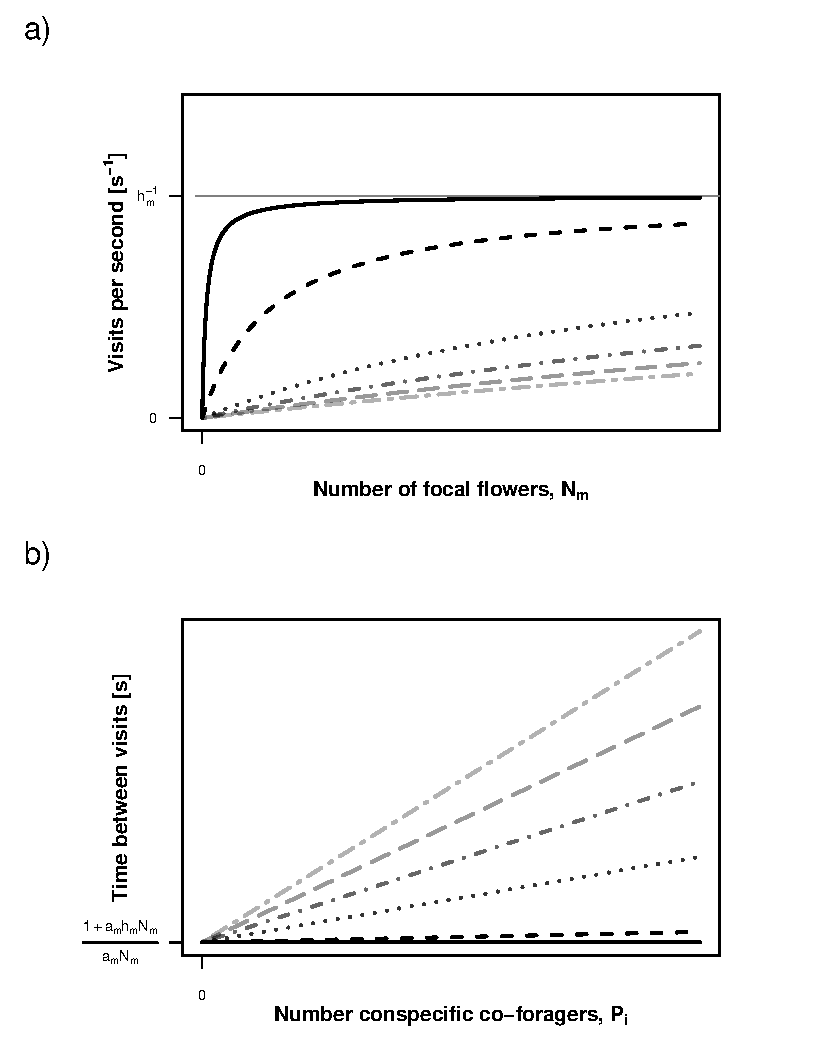
\includegraphics[height=0.7\textheight]{figures/chapter2_fig1.pdf}}
    \caption[Visualizing the mathematical relationship between visitation rate and time between visits.]{Visualizing the mathematical relationship between visitation rate and time between visits. a) Visitation rate as a function of the number of flowers $N_{m}$ (Eq~.\ref{lambda}). For a fixed number of co-foraging conspecific pollinators $P_{i}$ with no interference ($c_{i}$ = 0), no heterospecific pollinators present ($P_{j}$ = 0), and no other plants ($N_{n}$ = 0), the visitation rate saturates at at 1/$h_{m}$ (solid black line). As $c_{i}$ increases (dashed and dotted lines in lighter colours), the rate at which visitation rate reaches saturation decreases. b) Time between visits to a fixed number of focal flowers $N_{m}$ as a function of conspecific co-foragers $P_{i}$, also with $P_{j}$ = 0 and $N_{n}$ = 0 (Eq~.\ref{rho}). When $c_{i}$ = 0, the time between floral visits does not change with increasing pollinator abundance (solid black line). As $c_{i}$ increases, each co-foraging pollinator contributes more time to the time between floral visits (dashed and dotted lines in lighter colours as in a). }
    \label{fig:fig1}
\end{figure}

This general functional response framework allows us to quantify visitation rates under several experimental designs that might include scenarios (i) where floral abundances vary, (ii) where pollinator abundances vary, and (iii) under different environmental conditions.
For example, when there are observations of a focal pollinator and conspecific co-foragers visiting varying abundances of two plants, Eq.~\ref{rho} reduces to:
\begin{equation}
	\label{single_pollinator}
\rho_{i,m} = \frac{1}{a_{m}N_{m}}+ h_{m} + \frac{a_{n}h_{n}N_{n}}{a_{m}N_{m}} +\frac{c_{i}}{a_{m}N_{m}} (P_{i}-1)  \text{.}
\end{equation}

Note that to parameterize Eq.~\ref{single_pollinator}, we require independent variations of the abundances of both flowers \textit{and} of pollinators. However, it is also possible to adapt and fit a model based on our framework when only \emph{some} abundances change. For instance, if  the number of conspecific co-foragers $P_i$ is fixed, Eq.~\ref{single_pollinator} becomes:
\begin{equation}
	\label{single_pollinator_simple}
\rho_{i,m} =  h_{m} + \left ( \frac{1}{a_{m}} + \frac{c_{i}(P_{i}-1)}{a_{m}}\right ) \frac{1}{N_{m}} +  \left ( \frac{a_{n}h_{n}}{a_{m}}  \right ) N_{n} \frac{1}{N_{m}}
\end{equation}
which can be further simplified to:
\begin{equation}
	\rho_{i,m} = h_{m} + \gamma_{i,m} \frac{1}{N_{m}} + \delta_{i,n} N_{n} \frac{1}{N_{m}}  \text{.}
\end{equation}
Here the composite parameter $\gamma_{i,m}$ scales the impact of changes in focal floral abundances in the time between floral visits while $\delta_{i,m}$ scales the relative impact of changes in non-focal floral abundances. Since $\gamma_{i,m}$ includes encounter rates with flowers as well as the implicit impact of pollinator interference, these cannot be disentangled statistically without variation in $P_{i}$. Similarly, $\delta_{i,m}$ is a term that includes both the encounter rates with focal and with non-focal flowers.

On the other hand, when there are observations of different abundances of co-foragers visiting a fixed number of flowers of a single species, then Eq.~\ref{rho} becomes:
\begin{equation}
	\label{multiple_coforagers}
\rho_{i,m} = \frac{1+a_{m}h_{m}N_{m}}{a_{m}N_{m}} +\frac{c_{i}}{a_{m}N_{m}} (P_{i}-1) +\frac{c_{j}}{a_{m}N_{m}} P_{j}  \text{,}
\end{equation}
which can be further simplified to:
\begin{equation}
\label{interference_2}
		\rho_{i,m} =\alpha_{m} + \beta_{i,m} (P_{i}-1) + \beta_{j,m} P_{j} \,,
\end{equation}
where the composite parameter $\alpha_{m}$ sets a baseline of time between visits when there are no pollinator--pollinator interactions (i.e.\ the pollinator density-independent foraging outcomes), and the composite parameters $\beta_{i,m}$ and $\beta_{j,m}$ capture the  density-dependent changes to the time between visits to focal flowers. As above, both $\beta_{i,m}$ and $\beta_{j,m}$ incorporate both pollinator interference and encounter rates with flowers. Thus, an increase of times between floral visits (i.e.\ a decrease in floral visitation rates) could be the outcome of higher pollinator interference or decreasing encounter rates with flowers.

As a final example, both the density-dependent and density-independent terms can be inferred under different environmental conditions. For example, suppose we measure an enviomental variable $E$, and there are observations similar to those of Eq.~\ref{multiple_coforagers} but under different levels of the enviomental condition. Then, Eq.~\ref{interference_2} can be expanded into:
\begin{equation}
\label{interference_environment}
		\rho_{i,m} =\alpha_{m}+
		\alpha_{m,e} E +
	   (\beta_{i,m} + \beta_{i,m,e} E) (P_{i}-1) +
		(\beta_{j,m} + \beta_{j,m,e} E ) P_{j} \,,
\end{equation}
where $E$ is the value of the measured environmental variable (which can take continuous or discrete values), and the parameters with the subscript $e$ capture changes driven by abiotic conditions. For example, if $\beta_{i,m}$ quantifies the effect of conspecific pollinators, then $\beta_{i,m,e}$  quantifies how much the effect of conspecific pollinators changes under a certain abiotic condition. Written this way, both pollinator abundances and the enviomental conditions are the factors that determine the effect of pollinator--pollinator interactions.


\subsection*{Data}

In the following sections, we use our framework to parameterize and compare different models of floral visits with a unique foraging experiment. To do so, we examined data from a set of experiments that allowed us to tightly monitor the time  individual bumblebees spend between visits to artificial flowers, as well as the energy consumed per visit. During 2015 and 2016, we tracked the activity of commercial \textit{Bombus impatiens} (henceforth \textit{Bombus}) from Koppert Biological Systems (Howell, MI USA), inside a foraging chamber under (i) different richness and abundances of co-foragers and (ii) different levels of resource availability (iii) with and without pesticide exposure. These data  belong the ``Emory data set'', as described in \citet{ayers_statistically_2018}.

\subsubsection*{Experimental setup}

To monitor the activity of our focal species, our enclosure consisted of an array of artificial flowers that recorded the presence of a visiting bee an at the same time dispensed an automatic computer-controlled reward. The system was made up of 32 artificial flowers in four rows of eight flowers each distributed uniformly inside the chamber. The artificial flowers varied by color (blue, white, yellow, pink), scent, and sucrose concentrations (2.0 M, 1.5 M, 1.0 M, 0.5 M), in a way that yielded four distinct flower types. The automatic tracking of \textit{Bombus} individuals and co-foragers was done using mic3-TAG RFID 16 kbit tags (Microsensys GmbH, Erfurt, Germany) attached to each bee's thorax so as to not interfere with movement of flight.

Corresponding RFID tag readers embedded in each artificial flower recorded the presence of a bee (of any species) and activated an automatic reward of  10 $\mu$l unless the same individual had been recorded in that flower in the last 30 seconds, in which case no reward was conferred. If a different individual, of any species, visited the same flower, then the granting of a new reward depended on the floral refill time, or the time after which artificial flowers would dispense a new sucrose reward after a previous visit, a condition that we manipulated throughout the trials (see \textit{Foraging trials}). The sucrose reward was dispensed from a pipette tip embedded in the artificial flower, which was taken up by the bee’s proboscis through capillary action. Data suggests that the bees were almost always consuming the full reward offered by the artificial flowers (Fig.~1 Appendix A). This system allowed us to closely monitor the time between floral visits and energy consumption at the individual-bee level as well as resource availability using Arduino MEGA 2560 R3 hardware (Arduino LLC) and Processing software.


\subsubsection*{Foraging trials}

Foraging trials consisted of fasting the bees for one hour, transferring them to the foraging enclosure, and recording their behavior over 75 minutes. Before the experimental trials, we kept bees in separate training enclosures with artificial flowers identical to the ones in the experiment, except for the fact that training flowers were not computer controlled but delivered rewards \textit{ad libitum}. We simultaneously manipulated the richness and abundance of co-foragers, floral refill time, and the sub-lethal exposure to a common dose of a neonicotinoid pesticide as follows.

We manipulated the richness and abundance of co-foragers through a series of single-species and multi-species trials. In single-species trials, we varied the abundance of \textit{Bombus} to 4, 8 and 16 individuals foraging at the same time, with no other species present. In multi-species trials, we manipulated richness, or the number of species that were foraging at the same time as \textit{Bombus}. We examined the combinations of one to three additional bee species foraging at the same time as \textit{Bombus} while at all times holding total bee abundance constant at 16 individual bees. The three other species were another social bee species, \textit{Apis mellifera} (henceforth \textit{Apis}), and two solitary taxa, \textit{Osmia lignaria} and \textit{Megachile rotundata} (henceforth \textit{Osmia} and \textit{Megachile}). In multi-species trials, we used 8 \textit{Bombus} individuals for 2-species trials, either 5 or 6 \textit{Bombus} for 3-species trials, and 4 \textit{Bombus} for 4-species trials. We present a detailed description of the abundances of the other species during the experiment in Table 1 of Appendix A.

We also manipulated floral refill time to mimic different levels of resource availability since resource availability for the foraging bees decreases as refill time increases. The levels of floral refill time we examined were: instantaneous refill (0 seconds), intermediate refill (120 seconds), and delayed refill (540 seconds). We will refer to instantaneous refill (i.e.\ high resource availability) as the control condition.

Finally, we also manipulated bee exposure to a sub-lethal dose of neonicotinoid pesticide. While in the training enclosure, we fed individuals of all species subject to the pesticide treatment \textit{ad libitum} on a sucrose solution with a sub-lethal concentration of 10 $\mu$g/L of thiamethoxam ($C_{8}H_{10}CIN_{5}O_{3}S$, Sigma Aldrich); bees subject to the control condition were fed a sucrose solution without pesticide. For bees subject to pesticide treatment, the solution that contained pesticide was their only available sugar source. Thiamethoxam is applied to a wide range of crops \citep{maienfisch_chemistry_2001} and the concentration is consistent to what insects experience in the field \citep{blacquiere_neonicotinoids_2012}. We ran trials with either all exposed (of all species) or all unexposed bees to mimic exposure at the landscape level. We show a detailed description of the number of trials and replicates we performed in Tables 1 and 2 of Appendix A, as well as an explicit account of how the data was cleaned for analysis.

\subsection*{Analysis}

\subsubsection*{Models of times between floral visits}

Given our framework and our very detailed data-set, we were able to contrast different hypotheses regarding how pollinators forage and interact, using \textit{Bombus} as our focal species. Instead of testing \textit{all} possible hypotheses of how co-foragers, resouce availability and pesticide exposure influence the times between floral visits, we tested three relatively simple hypotheses: (i) \textit{Bombus} individuals forage unaffected by the presence of co-foragers or by environmental conditions, (ii) only co-foragers modify how \textit{Bombus} forages but environmental conditions do not, and (iii) environmental conditions modify how individuals forage alone and in the presence of other foragers. Our modelling aim was not to get a detailed prediction of the dynamics governing the experimental system, but rather to show that the modelled principles are sufficient to explain times between floral visits, following a demonstration modelling approach to reveal potential explanatory generalities \citep{evans2013simple}.


If we map our functional response framework to our experimental setup, we can describe the functional response of the focal \textit{Bombus} individuals with Eq.~\ref{interference_2}. Our hypotheses can then be tested across different foraging models that equate to further extensions or simplifications of Eq.~\ref{interference_2}. If the presence of co-foragers and environmental conditions have no effect on the times between visits across experiments, then a density-independent rate will be sufficient to describe the data:
 %
\begin{equation}
    \rho_{i}= \alpha \,.
    \label{null}
\end{equation}
 %
We call this our \textit{null} model. Note that since in our experiment floral abundances remained constant, we did not explore how changes in densities of different flower types changed foraging rates. Rather, we modelled how long \textit{Bombus} individuals would take between visits to all of the artificial flowers, regardless of the type of flower. Thus, for simplicity we dropped subscripts on terms that depended on flower types.

On the other hand, if co-foragers interact with each other but visitation is unaffected by the abiotic conditions, then an equation similar to Eq.~\ref{interference_2} that only considers the effect of co-foragers would best describe the times between floral visits. We call this the \textit{interference} model:
\begin{equation}
\label{interference_3}
		\rho_{i} =\alpha + \beta_{i} (P_{i}-1) + \sum_{j}\beta_{j}P_{j} \,.
\end{equation}

Finally, if the abiotic treatments modify how \textit{Bombus} forages with and without co-foragers, similiar to Eq.~\ref{interference_environment}, we would expect the times between visits to be a function of the abundance of co-foragers, level of resource availability ($R$) and pesticide exposure ($E$), we call this the \textit{treatments} model:
\begin{equation}
\label{treatments}
\rho_{i} =\alpha + \alpha_{r} R+   \alpha_{e}E +  \beta_{i} (P_{i}-1) +  \beta_{i,r} (P_{i}-1) R +  \beta_{i,e} (P_{i}-1) E        + \sum_{j}\beta_{j}P_{j}  +  \sum_{j}\beta_{j,r}P_{j}R +  \sum_{j}\beta_{j,e}P_{j}  E \,.
\end{equation}
Here the subscripts  $r$ and $e$ denote the parameters that estimate the effect of $R$ and $E$, respectively. In our case, $R$ is a continuous variable that corresponds to the floral refill time (i.e.\ goes from 0 to 540 seconds) and $E$ is a dummy variable to indicate pesticide exposure (i.e.\ $E = 0$ when bees are subject to the control treatment, and $E=1$ when bees were exposed to the pesticide treatment). The subscripts we used are consistent with the nomenclature of the density-independent and density-dependent terms described previously. Note that in our data, not all co-foraging species were tested under all experimental conditions (Table 1 Appendix A). Therefore, we did not model the three-way interaction between species identity, pesticide exposure and resource availability.


\subsubsection*{Statistical analyisis}

To  infer the parameters of Eqs.~(\ref{null}-\ref{treatments}), we fit non-linear hierarchical models with a Bayesian framework using Hamiltonian Monte Carlo (HMC) methods. We provide the details of our statistical analyisis in Appendix A. We fit our  models using the function  \textit{brm} from the package \textit{brms} \citep{burkner_advanced_2017} in the statistical program \textsc{R} (version 3.4.2) \citep{Rcore}. We ran four chains with a warm up of 3000 iterations and 2000 sampling iterations, using weakly informative priors and a maximum treedepth of 13 and an adapt delta of $0.99$. We determined convergence when trace plots were well mixed and stationary and when the Gelman-Rubin convergence diagnostic (Rhat) was less than 1.05 for all parameters \citep{vehtari_rank-normalization_2020}.

We compared the fits of  Eqs.~(\ref{null}-\ref{treatments}) to each other using the the Wanatabe-Akaike information criterion (WAIC) to determine which of the hypotheses encoded within the models best predicts out of sample times between floral visits. WAIC provides a measure for model fit that is penalized for the number of model parameters, and the best fit model in terms of out of sample predictions is the one with the lowest WAIC value. Additionally, we calculated Akaike weights for each model, which can be  interpreted as an estimate of the probability that the model will make the best predictions of new data based on the the set of models considered. We did model comparisons using 500 samples from the posterior distribution, and we defined best-fit models as those with the lowest WAIC and an Akaike weight greater than 0.9 \citep{mcelreath_statistical_2018}.

\section*{Results}

Model comparison using Wanatabe-Akaike information criterion (WAIC) showed that the \textit{treatments} model was the best-fit model for explaining the data by a wide margin (Table~\ref{tab:waic}). The \textit{treatments} model had the lowest WAIC score and received all of the Akaike weight, which means it had the highest probability to make the best predictions of new data compared to the two other models considered. Model comparison therefore showed not only that co-foraging pollinator abundances systematically modified the times between floral visits, but also that resource availability and pesticide exposure modified how bumblebees foraged alone and with other species present.

\subsection*{Density-independent effects}

The parameters of the \textit{treatments} model allowed us to make predictions beyond the pollinator densities manipulated during the trials since it estimated density-independent effects as the intercept. Without any co-foragers present, predictions using the \textit{treatments} model confirmed that both low resource availability and sub-lethal exposure to pesticide increased the time between floral visits (Fig.~\ref{fig:fig2}). Predictions made at low resource availability and under pesticide exposure (Fig.~\ref{fig:fig2}d) showed that a bumblebee foraging alone would spend on average 90 seconds more between floral visits when compared to predictions made at high resource availability and under no pesticide exposure (Fig.~\ref{fig:fig2}a); this equates to a near doubling of the amount of time between floral visits. Consequently, over the course of a 75 minute experiment, an average bumblebee foraging alone would make 15 fewer floral visits if there was low resource availability and it had been exposed to pesticide.

\begin{table}[H]
\centering
\caption[Model comparison table]{Model comparison table. WAIC (Widely Applicable Information Criteria) penalizes models for parameters, and the lowest WAIC reflects the best-fit model. pWAIC is the effective number of parameters and provides information on how flexible each model is in fitting the sample. Akaike Weight for each model is an estimate of the probability that the model will make the best predictions of new data based on the the set of models considered.}
\label{tab:waic}
\begin{tabular*}{\textwidth}{l @{\extracolsep{\fill}} ccc}
\toprule
model        & WAIC     & pWAIC  & Akaike weight        \\ \midrule
\textit{treatments}   & 413322.5 & 2386.6 & 1.00  \\
\textit{interference} & 414462.5 &  2135.6 & < .002 \\
\textit{null}         & 416063.6 &  1769.6  & < .002\\ \bottomrule
\end{tabular*}
\end{table}

As shown in the intercepts of Fig.~\ref{fig:fig2}a and c, we also found that the time between floral visits decreased as resource availability increased (i.e.\ the time between floral refill decreased). Predictions made at high resource availability (0 seconds between floral refill) showed that an average bumblebee would make 7 more floral visits over the course of an experiment than it would at low resource availability (540 seconds between floral refill).

\textit{Density-dependent effects}

We found that the time between floral visits for a focal pollinator changed consistently as a function of the identity and abundance of the co-foragers (Fig.~\ref{fig:fig2}). All of the species examined could potentially interfere with a focal \textit{Bombus} individual by increasing the time between floral visits, but the extent of the interference effect depended on the environmental context bees experienced.

Under control conditions (i.e.\ no pesticide exposure and high resource availability), increasing abundances of \textit{Bombus}, \textit{Osmia}, and \textit{Megachile} all increased the times between visits (and therefore decreased the visitation rate) to a similar extent (Fig.~\ref{fig:fig2}a). However, \textit{Apis} had an opposite effect under control conditions as increasing its density \emph{decreased} the times between floral visits. Thus, when there was high resource abundance and no pesticide exposure three of the species (including conspecifics) had an interference effect. However, as environmental conditions changed, so did these interference effects. For example, increasing abundances of \textit{Apis} changed from decreasing times between visits to increasing them when there was either pesticide exposure or low resource availability (Fig.~\ref{fig:fig2}).



\begin{figure}[H]
    \centerline{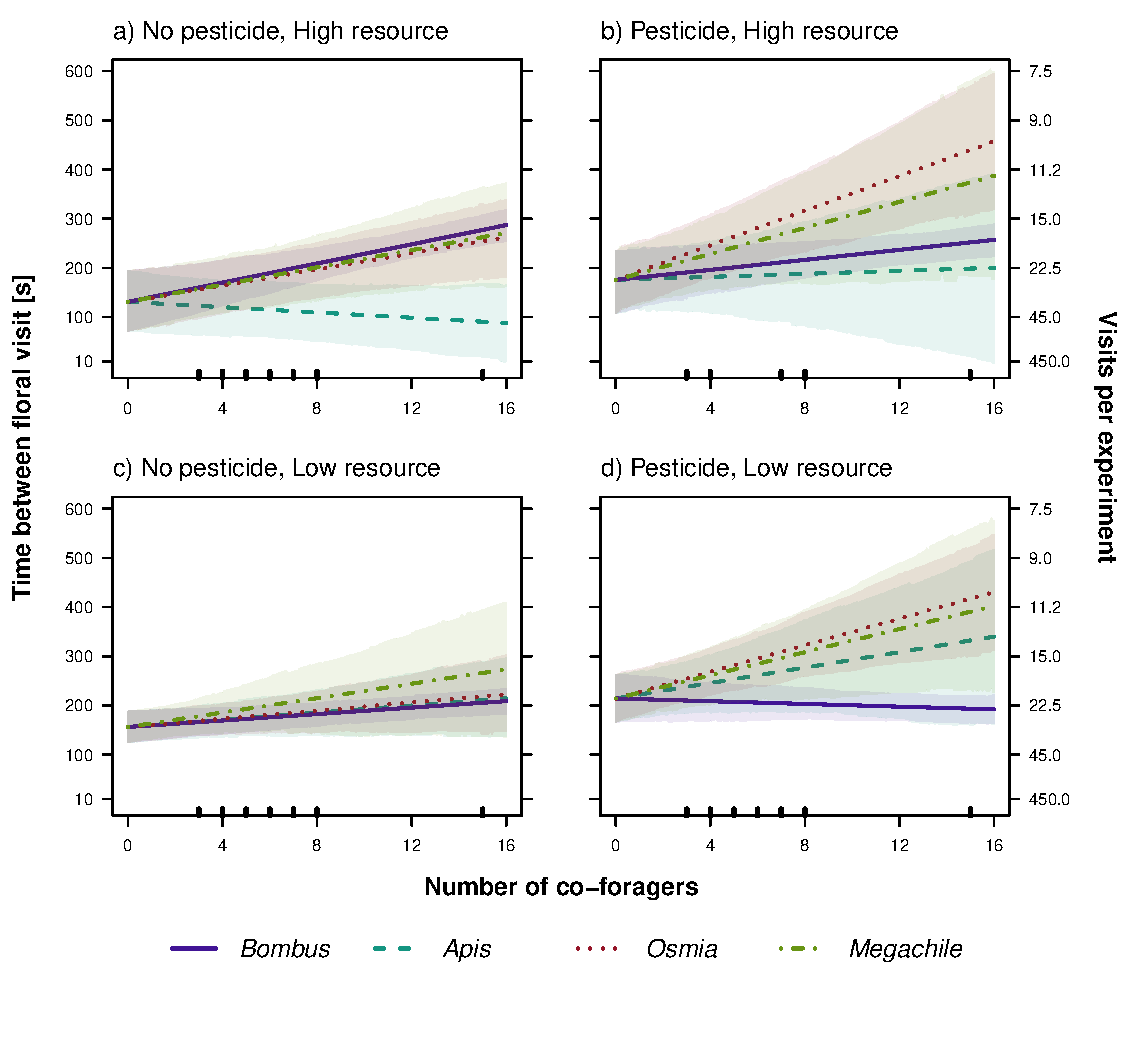
\includegraphics[height=0.7\textheight]{figures/chapter2_fig2.pdf}}
    \caption[Model predictions of how the time between floral visits changed as the number of co-foragers increased and under different environmental conditions]{ Model predictions of how the time between floral visits changed as the number of co-foragers increased and under different environmental conditions. Each color and line type correspond to a different co-forager. Lines represent predictions using the median parameter values of the \textit{treatments} model for the average focal individual. The shaded areas correspond to the 90\% highest posterior density interval (HPDI). High resource availability corresponds to 0 seconds between floral refill, and low resource availability to 540 seconds between floral refill (the maximum used during the experiments). Ticks along the x-axis indicate the actual co-forager abundances examined during the experimental trials. On the right y-axis and to help interpretation, we show how many visits per 75 minute experiment would be expected for the corresponding times between floral visits.}
    \label{fig:fig2}
\end{figure}{}

To better disentangle the species-specific response of interference to environmental variables, we estimated the time contributed by a single co-forager individual of each species to the total times between floral visits as resource availability increased (Fig.~\ref{fig:fig3}) and with the exposure to a neonicotinoid pesticide (Fig.~\ref{fig:fig4}). That is, given the posterior distribution of the fixed effects, we calculated how total times between floral visits changed due to the contribution of a single individual of each species under different environmental conditions. Note that due to the inverse relationship between time between floral visits and resource availability, Fig.~\ref{fig:fig3} shows decreasing times between floral refill.

We found that, as resources became more abundant (or the time between floral refill decreased), interference by \textit{Bombus}, \textit{Osmia}, and \textit{Megachile} increased (Fig.~\ref{fig:fig3}). In particular, the time contributed by a conspecific individual almost tripled when resource availability changed from low to high (Fig.~\ref{fig:fig3}a). For the majority of the species examined, interference was strongest when there was high resource availability, and its effect weakened as resources became more scarce. In contrast, as resources became more abundant, the contribution of an additional individual of \textit{Apis} to the time between floral visits decreased. Indeed, our predictions using median parameter values showed that an individual of \textit{Apis} went from creating net decreases in visitation rate at low resource availability to creating net increases in visitation rate at high resource availability (Fig.~\ref{fig:fig3}b). However, the predictions using the 90\% highest posterior density interval (HPDI, or the narrowest interval containing the specified probability mass \citep{mcelreath_statistical_2018}) for \textit{Apis} included competitive and facilitative outcomes at all levels of resource availability. Thus, even though on average \textit{Apis} individuals had a facilitative effect as resources became more abundant, we predicted some competitive effects as well when making predictions using the full posterior distribution.

In contrast to resource availability, pesticide exposure tended to increase the strength of pollinator interference for all species except \textit{Bombus}(Fig.~\ref{fig:fig4}). That is, when all of the bees had been exposed to pesticide, increasing heterospecific abundances of pollinators generally decreased floral visitation rate because individuals contributed positively to the times between floral visits. Conspecifics, however, had the opposite effect: pesticide exposure decreased the strength of pollinator interference (Fig.~\ref{fig:fig4}).


\begin{figure}[H]
    \centerline{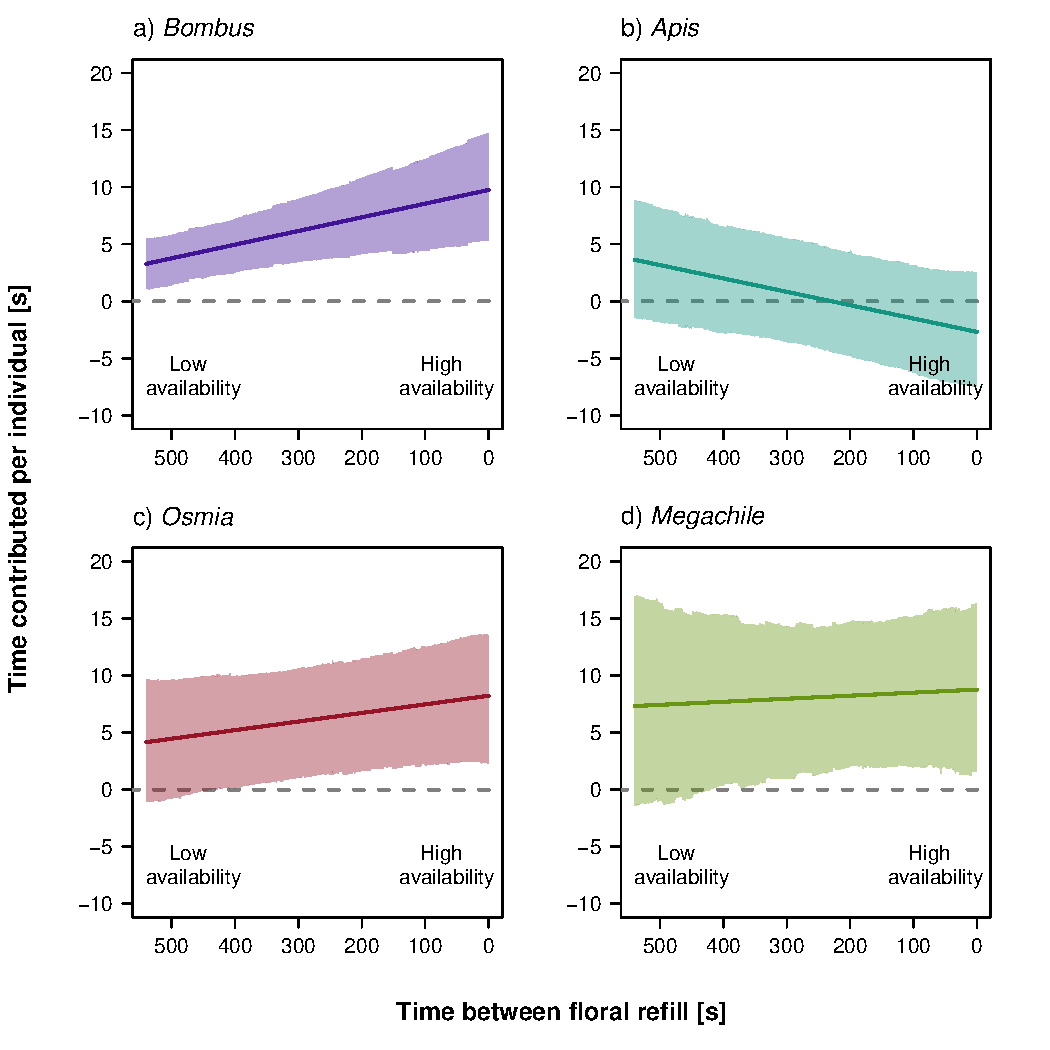
\includegraphics[height=0.7\textheight]{figures/chapter2_fig3.pdf}}
    \caption[Model predictions of the effect an individual co-forager had on the time between visits of \textit{Bombus} as resource availability increased]{Model predictions of the effect an individual co-forager had on the time between visits of \textit{Bombus} as resource availability increased and when there was no pesticide exposure. Each panel estimates the contribution of an individual co-forager from each of the four co-foraging species from our study. Solid lines represent the predictions made with the median parameter values of the \textit{treatments} model for the average focal individual whereas the shaded areas correspond to the 90\% highest posterior density interval (HPDI). To help interpretation, we provide the mapping between low and high resource availability and time between floral refill in each panel.  }
    \label{fig:fig3}
\end{figure}{}





\begin{figure}[H]
      \centerline{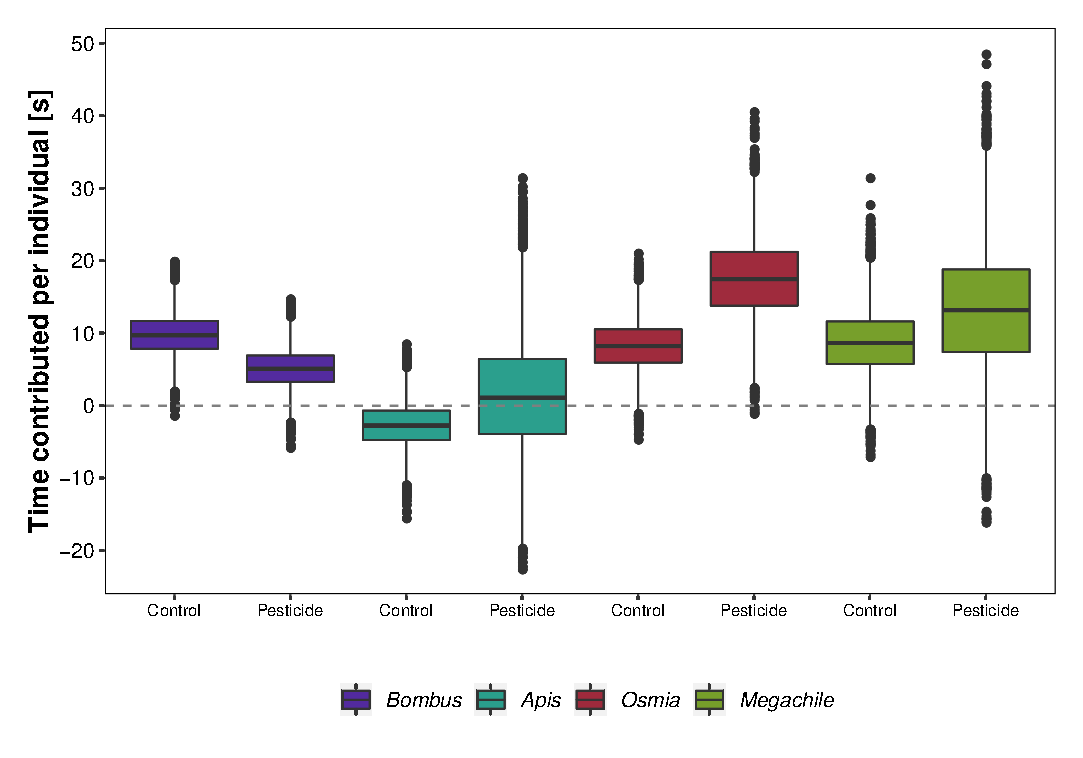
\includegraphics[width=1\textwidth]{figures/chapter2_fig4}}
    \caption[The effect an individual co-forager had on the time between floral visits]{ The effect an individual co-forager had on the time between floral visits when it had not been exposed to pesticide at high resource availability (Control), and when it had been exposed to a sub-lethal dose of neonicotinoid pesticide and at high resource availability (Pesticide). Each color corresponds to the different species of co-foragers. Each box plot extends from the first to third quantiles of the corresponding posterior distribution of parameter values, and the line inside the the box indicates the median. The upper whisker extends to the largest value no further than 1.5 times the inter-quantile range (IQR, or the distance between the first and third quartiles); the lower whisker extends to the smallest value at most 1.5 times the IQR. Data beyond the end of the whiskers are determined to be outliers and are plotted individually with solid black points.}
    \label{fig:fig4}
\end{figure}

\section*{Discussion}

%Paragraph to summarize the most important results that will be discussed below
We applied our functional response framework to illustrate how both environmental context and pollinator--pollinator interactions can substantially change the number of visits a pollinator will make. Our model predictions showed that when a pollinator was foraging alone, conditions such as low resource availability and exposure to a sub-lethal dose of pesticide decreased the visits made to flowers. However, the same environmental conditions could have opposite effects on pollinator--pollinator interactions; for most species examined, interference was strongest when there was high resource abundance, and pollinator interference decreased as resources became scarcer (except for \textit{Apis}). Finally, we found a density-dependent response to pesticide exposure since, for all co-foraging species except \textit{Bombus}, exposure to pesticide increased the sensitivity to individuals of other co-foraging species. On the whole, our results make clear that the question is not whether or not pollinators interfere with each other, but under what conditions they do so.


\subsection*{Resource abundance}

%The effects of resource abundance on a pollinator foraging alone
When resources are scarce, it has been previously documented that bumblebees make fewer visits to flowers than in rich-resource areas \citep{heinrich_bumblebee_2004,westphal_foraging_2006}. Our predictions agreed on the effect of low resource availability when a pollinator is foraging \textit{alone} (Fig.~\ref{fig:fig2}). For bumblebees, high resource availability can be associated with mass-flowering \citep{westphal_mass_2003}, and other studies have shown that net benefits are increased when bumblebees concentrate their efforts in areas of rich nectar resources while moving rapidly through depleted areas \citep{heinrich_resource_1979}.
%Thus, the increase in visitation rates with resource availability could be explained as a systematic exploitation of the most rewarding resources \citep{pyke_optimal_1978}.
%On the other hand, \citet{jha_resource_2013} found that bumblebees tend to increase visits in patches with high floral diversity, not density. Since the flower distribution (color, scent, and sucrose concentration) remained constant in our foraging chamber, we could only assess how resource abundance (measured in floral refill time) modifies foraging behavior.

%The effects of resource abundance on a pollinator foraging with other species
In contrast, the role of resources was reversed when a bumblebee foraged at the same time as other species. For most of the species examined, interference was strongest when resources were most abundant (Fig.~\ref{fig:fig3}). Recall that in our modeling framework an increase of times between floral visits can be caused by many different mechanisms. For example, we found with $\beta_{i,r}$ that the effect of conspecifics decreased as resources became more scarce. This decrease could be due to a decrease in overt interference, $c_{i}$, or to a lower encounter rates with flowers $a_{m}$. However, observations of bees during the experiments offer some potential insights into this question. First and foremost, we never observed obvious aggressive interactions between bee individuals in the foraging arena. Instead, interference appears to have been driven by avoidance of flowers due to visual and/or olfactory cues presented by other bee individuals. The response to these cues was clearly context dependent. For example, while we did not specifically test learning within individual bees, they may have learned within the course of a trial that a visual or olfactory cue of another individual at a flower signaled that the flower was unlikely to be rewarding (in the case of delayed floral refill) or that the cues were not related to rewards (in the case of instantaneous floral refill). Indeed, overt interference has not been observed in bumblebees \citep{heinrich_resource_1976, heinrich_bumblebee_2004}, but bumblebees have been documented to have avoidance behavior when foraging with other species \citep{morse_resource_1977, inouye_resource_1978} and  are able to detect and reject flowers which have been visited by other \textit{Bombus} species using scent \citep{goulson_foraging_1999}.

Additionally, different bee species behaved differently in the experiments and the contribution to the times between floral visits we found (positive and negative) was also reflective of competitor species identities. For example, \textit{Apis} individuals generated net increases in floral visits by decreasing the time between floral visits under high resource availability. This may be because honey bees were not particularly active in foraging and may have spent more time outside of flowers, which could have led to essentially an overall decrease in competition for \textit{Bombus}. Previous studies have found that interspecific interactions between honeybees and other species can sometimes result in an increase in pollination efficiency \citep{greenleaf_wild_2006}. In contrast, \textit{Megachile} individuals also had low foraging rates, but based on observations may have spent more time in and near flowers, potentially leading \textit{Bombus} individuals to avoid those flowers and increasing interference despite low foraging rates. Changes in bee foraging behavior have been shown to be species-specific before \citep{briggs_competitive_2016}, and it remains an exciting and open challenge to fully understand how they explicitly depend on environmental conditions.

% The effects of pesticide in general
\subsection*{Pesticide exposure}

Our results were also consistent with previous studies that saw a decrease in floral visits when pollinators are exposed to a sub-lethal dose of neonicotinoid pesticide \citep{gill_chronic_2014, henry_common_2012, stanley_chronic_2016, mommaerts_risk_2009}. Neonicotinoid pesticides bind strongly to nicotinic acetylcholine receptors in the central nervous system of insects \citep{goulson_review_2013}. At sub-lethal doses, this creates difficulties for memory and learning \citep{henry_common_2012}, as well as compromises navigation skills \citep{desneux_sublethal_2007}. Unsurprisingly, exposure to thiamethoxam increased the times between floral visits when a bumblebee was foraging alone and with the addition of individuals  of all of the heterospecific pollinators (Fig.~\ref{fig:fig2} \&\ref{fig:fig4}). For conspecifics, pesticide exposure weakened the effect of conspecific interference. That is, relative to the control conditions, foraging with conspecific individuals still resulted in a net decrease of floral visits but to a lesser extent. Thus, the general effect of sub-lethal exposure to a neonicotinoid pesticide is to decrease floral visits via both by density-dependent and density-independent mechanisms.

 %Given our experimental set-up, our results portray how we would expect bees to behave when all foraging species have been exposed to pesticide.

\subsection*{Experimental limitations }

In our study, the highly controlled experimental setup allowed us to tightly monitor bee behavior and thus explicitly quantify pollinator interference and its relationship with experimental treatments. However, the artificial environment  might not accurately capture how bees forage in the wild. For example, bumblebees could not leave low resource areas and concentrate their efforts in less depleted areas as they are prone to do \citep{heinrich_bumblebee_2004}. Furthermore, the non-focal species were not as active as \textit{Bombus} during the trials, which might further change how interference operates. Thus, the results presented here should be considered in the context of a controlled foraging experiment. This notwithstanding, we directly quantified behavioral changes driven by the presence of other pollinator species into pollinator functional responses, which has rarely been done.

\textit{Consequences of pollinator--pollinator interactions}

In this study we focused on the functional responses of pollinators, and did not quantify their numerical responses \citep{morris_benefit_2010}. Without knowing the numerical responses of the populations involved, we can not fully understand the dynamic consequences of pollinator--pollinator interactions \citep{revilla2015numerical}. However, our results do provide insights of how interference might affect mutualistic communities. Empirical and theoretical studies suggest that how often pollinators visit plants is a good predictor of the strength of the interaction, for both pollinators and plants involved \citep{vazquez_interaction_2005,vazquez_strength_2012}. Indeed, in our experimental system the number of floral visits was a good predictor of the energetic gains for bees, since bees seemed to almost always consume the full reward offered by artificial flowers (Fig~.\ref{fig:flower_type}, Supporting Information). Thus, from the point of view of pollinators, foraging with other species can be disadvantageous under certain conditions. For example, if high resource abundance made the other species more active, \textit{Bombus} individuals might spend longer between flower visits because they are trying to avoid flowers that have already been visited. However, from the plant's perspective, receiving visits from a diverse pollinator assemblage can produce more stable plant reproduction \citep{sahli2006characterizing}, and greater competition tends to make bees increase floral fidelity, which also enchances plant fitness \citep{brosi_single_2013}. Much like plant diversity \citep{bruninga2016role}, our results show that pollinator diversity does not always have straightforward consequences on the populations involved.


\subsection*{Conclusion}

The impact of interactions between pollinators in natural communities it is still poorly understood. In this study, we argue that in order to understand when and why those interactions change the course of plant and pollinator populations, we should also determine the environmental context in which they occur. Importantly, our study provides a theoretical framework to do so, coupled with a highly controlled foraging experiment to show how drastically abiotic conditions can change the outcomes of pollinator--pollinator interactions. By incorporating intra-guild interactions into pollinator functional responses, our study opens up an urgent avenue to study the consequences of species loss and enviomental change in natural communities. It is critical to determine just how prevalent interference or facilitation between pollinator species is in nature, in order to further understand how species loss could affect pollinator populations. We believe our study gives ecologists the theoretical and statistical tools to quantify the effects of other species both in experimental and observational studies, and contributes to closing the gap between the mutualistic and predator--prey literatures.


%(Fig.~\ref{fig:fig1}).

\printbibliography
\end{refsection}
 % Chapter 3
\begin{refsection}
\chapter{The interplay of environmental conditions, parameter sensitivity and structural sensitivity in predictions of species coexistence} % Main chapter title
\label{Bayesian_competition}

\noindent Alba Cervantes-Loreto\textsuperscript{1}, Abigail Pastore \textsuperscript{2}, Christopher R.P.\ Brown\textsuperscript{1},Michelle L.\ Maraffini\textsuperscript{1},Clement Aldeber\textsuperscript{3},Clement Aldeber\textsuperscript{3},Margaret M.\ Mayfield\textsuperscript{2},Daniel B.\ Stouffer\textsuperscript{1}

\begin{enumerate}
    \item Centre for Integrative Ecology, School of Biological Sciences, University of Canterbury, New Zealand
    \item School of Biological Sciences, University of Queensland, Brisbane, Australia
    \item Aix Marseille Univ., Université de Toulon,  Marseille, France
\end{enumerate}

\section*{Abstract}


Predicting the outcome of competitive interactions among species that share resources is central to our current understanding of diversity maintenance. However, we have little information about how robust are predictions of species coexistence. This limitation is partly because several sources of uncertainty are often ignored when making predictions. Here, we introduce a mathematical and statistical framework to simultaneously explore how different models, environmental contexts and parameter uncertainty change the probability of predicting species coexistence.  Using a set of pairwise competition experiments of annual plants, we provide direct evidence that seemingly subtle differences between models led to predictions of both coexistence and competitive exclusion based around the exact same experimental data. We also show that the effects of environmental context-dependency and parameter uncertainty on predictions of species coexistence are not independent of the model formulation used to describe species dynamics. Our work suggests that predictions of species coexistence and extrapolations made from them are particularly vulnerable to change due to the three sources of uncertainty we studied.

\section*{Introduction}


The effects species have on one another are the result of multiple processes that often act simultaneously. In the case of competition between plants, examples include the depletion of local resources in the soil \citep{dybzinski2007resource, craine2013mechanisms},  visits from shared pollinators \citep{lanuza_opposing_2018}, or the frequency and intensity of disturbance events \citep{pickett1980non, villarreal2009species}. Notwithstanding their importance, fully including all such phenomena in the study of plant dynamics is often impractical. Hence, it is more straightforward to treat these processes implicitly and model the relationship between interacting species phenomenologically, for example by fitting models that describe how the densities of intraspecific and interspecific neighbors change plant fitness and growth \citep{case1999illustrated, adler2018competition}.


Despite their ``necessary incompleteness'', phenomenological models can accurately reproduce the observed data in various natural systems and contexts \citep{bolker_ecological_2008}. Perhaps more importantly, they are useful tools with which to make predictions that extend beyond the phenomena they describe. Such predictions are possible because of the implicit assumption that models that reproduce the observed data faithfully also capture how the studied system operates \citep{marquet2015importance}. For example, models that describe the effects neighboring plants have on each other can be used to make quantitative predictions about changes of biomass in the system \citep{godoy2020excess, lai2020role} or qualitative predictions such as whether or not co-occurring plant species can coexist \citep{levine2009importance, zepeda2019fluctuation}.

% some references you might be looking for in terms of "...operates" above are:
% Klir, G. J., 1985. Architecture of Systems Problem Solving. Plenum Press, New York, NY, USA.
% Zeigler, B. P., Praehofer, H., and Kim, T., 2000. Theory of Modeling and Simulation. Academic Press, San Diego, CA, USA.
% Marquet, P. A., Allen, A. P., Brown, J. H., Dunne, J. A., Enquist, B. J., Gillooly, J. F., Gowaty, P. A., Harte, J., Hubbell, S. P., Okie, J. G., Ostling, A., Ritchie, M., Storch, D., and West, G. B. 2015. On the importance of first principles in ecological theory development. BioScience 65:342–343.

The practicality of phenomenological models of plant competition, however, is a double-edged sword. Indeed, predictions made with them are subject to uncertainty arising from many distinct sources. One of these is environmental context dependency, or the extent to which the outcomes of species interactions change as a function of the abiotic conditions species experience \citep{chamberlain_how_2014}. Many studies have documented how the sign and magnitude of species interactions change with environmental conditions, such as interspecific interactions between plants switching from competitive to facilitative in harsh environments \citep{callaway_positive_2002, maestre2005change, brooker2008facilitation,maestre2009refining}, changes to the identity of the competitive superior plant species as abiotic conditions change \citep{poorter1986growth, dybzinski2007resource}, or variations in interaction strength between plants along environmental gradients \citep{bimler_accurate_2018, villarreal2009species, lanuza_opposing_2018}. Extrapolations from phenomenological models of plant competition can therefore be highly specific to the set of conditions under which models were parameterized \citep{bimler_accurate_2018}.


Model-based predictions are also subject to two forms of uncertainty that arise from the use of models themselves: parameter sensitivity and structural sensitivity. Parameter sensitivity refers to the sensitivity of model outputs to variation in parameter values \citep{flora_structural_2011}, and exploring it constitutes a routine analysis in the domain of the biological sciences \citep{jorgensen2001fundamentals}. On the other hand, structural sensitivity characterizes how  mathematical expressions that have similar phenomenological behavior can produce qualitatively different outcomes \citep{flora_structural_2011,myerscough1996stability,aldebert2018community}. Parameter and structural sensitivity are often intertwined \citep{wood1999super}, and both have been shown to drastically change model predictions in a vast array of biological systems \citep{flora_structural_2011, wood1999super, poggiale2010far, fussmann2005community,  aldebert2018community}.

The interplay between environmental context dependency, parameter sensitivity, and structural sensitivity is rarely explored simultaneously, and to the best of our knowledge  has never been explicitly explored in the case of models of density dependence in plant performance. In this study, we therefore aim to understand how these three sources of uncertainty change predictions of a widely studied and vastly important ecological process: species coexistence. We focused our analysis on annual plants, which is a common natural system used to study species coexistence \citep{mayfield2017higher, godoy_phenology_2014,levine2009importance, zepeda2019fluctuation}. We assessed the empirical relevance of the three different sources of uncertainty by making coexistence predictions based around data from a competition experiment between two annual plants conducted in two contrasting abiotic conditions. Our analyses provide evidence that uncertainty can radically change predictions made from a simple competition experiment, and highlights the importance of incorporating uncertainty from different sources in predictions made with phenomenological models.

\section*{Methods}

We will first provide a mathematical description of how to make and interpret coexistence predictions made with a single phenomenological model of two species of annual plants growing in proximity to each other. We then expand our framework to introduce an alternative phenomenological model of plant density dependence, and show how our framework can be used to make predictions using a different model per species. Second, we describe how to use a Bayesian framework to parameterize the  aforementioned  phenomenological models  to data from a set of competition experiments between two annual plants growing in two contrasting abiotic conditions. Finally, we describe how we simultaneously explored structural sensitivity, parameter sensitivity, and environmental context dependency to make predictions of species coexistence.


\subsection*{Model-based predictions of species coexistence }

We used the Cohen model \citep{cohen1966optimizing,watkinson_density-dependence_1980} to describe annual-plant population dynamics and as the starting point for our model-based predictions of species coexistence. This model predicts the number of seeds $N_{i,t+1}$ from species $i$ in year $t+1$ with:
\begin{equation}
\label{annual_plant}
    N_{i,t+1}= (1-g_i)s_{i} N_{i,t}  + g_{i} N_{i,t}F_{i,t}\,,
\end{equation}
which is a function of prior number of seeds in the soil ($N_{i,t}$) that survive that year in the seed bank (as weighted by $s_{i}$, the fraction of non-germinating seeds that survive in the soil), and the seeds that germinate (described by $g_i$) multiplied by the number of viable seeds produced per seed germinated, often called their realized fecundity ($F_{i,t}$). The realized fecundity of species \textit{i} can be accurately described by many different phenomenological forms \citep{law_response-surface_1987, godwin2020empiricist}. Note that the phenomenological descriptions of $F_{i,t}$ generally try to capture the density dependence of plant performance on the number of conspecific and heterospecific neighbors, but do not necessarily imply a hypothesis about the mechanisms underpinning this density dependence.

As an example, $F_{i,t}$ can be given by the Beverton--Holt model \citep{beverton1954notes}, which in a two-species context equals:
 \begin{equation}
 \label{Beverton-Holt}
    F_{i,t} = \frac{\lambda_{i}}{1 + \alpha_{ii}g_{i}N_{i,t} + \alpha_{ij}g_{j}N_{j,t}}\,.
\end{equation}
In this model, the per germinant fecundity of species \textit{i} in the absence of competition is described by the parameter $\lambda_{i}$, while the numbers of germinants of species $i$ and $j$ in year $t$ are given by $g_{i}N_{i,t}$ and $g_{j}N_{j,t}$, respectively. The density-dependent effects are captured by the interaction coefficients $\alpha_{ii}$ and $\alpha_{ij}$, which describe the interaction strength of conspecifics and heterospecifics, respectively. The Beverton--Holt model is a commonly used phenomenological model to make coexistence predictions and can be easily parameterized with empirical observations of annual plants growing in proximity to each other \citep{godoy_phenology_2014, godoy_phylogenetic_2014, levine2009importance}.

\subsubsection*{Coexistence predictions}

From the population dynamics that result from using Eqn.~\ref{annual_plant} and estimates of the relevant parameters of Eqns.~\ref{annual_plant} and ~\ref{Beverton-Holt},  it is possible to predict if a pair of species can coexist. Multiple approaches exist to predict species coexistence \citep{chesson_general_2000, chesson_updates_2018, barabas_chessons_2018, saavedra2017structural, letten_linking_2017}. One of them is to directly evaluate, given the competitive constraints each species experiences, if the set of species intrinsic growth rates is feasible \citep[i.e., if there exists an equilibrium point under which both species have positive abundances;][]{rohr_structural_2014, saavedra2017structural}. To do so, it is necessary to derive the equations determining the equilibrium density for each species, which for species $i$ is found at:

\begin{equation}
\label{equilbrium}
  \frac{N_{i,t+1}}{N_{i,t}}  = (1-g_{i})s_{i} + \frac{g_{i}\lambda_{i}}{1 + \alpha_{ii}g_{j}N_{i}^{*} + \alpha_{ij}g_{j}N_{j}^{*}}  = 1 .
\end{equation}

This equilibrium condition can be arranged to provide a linear equation in terms of seed densities:
\begin{equation}
\label{bh_equilibrium}
    -1 + \left( \frac{g_{i}\lambda_{i}}{1-(1-g_{i})s_{i}} \right) = \alpha_{ii}g_{i}N_{i}^{*} + \alpha_{ij}g_{j}N_{j}^{*}.
\end{equation}
For reasons that will hopefully become clear later, Eqn.~\ref{bh_equilibrium} can be rewritten as:
\begin{equation}
  \label{growth_competition}
  r_{i} = \alpha_{ii}g_{i}N_{i}^{*} + \alpha_{ij}g_{j}N_{j}^{*},
\end{equation}
where $r_{i}$ is the intrinsic growth rate of  species $i$. Note that $r_{i}$ is a composite parameter that depends on the values of $s_{i}$, $g_{i}$, and $\lambda_{i}$. Equivalent expressions for species $j$ can be derived from its equilibrium condition. The combined two-species equilibrium condition is:
\begin{equation}
\begin{bmatrix}
r_{i} \\
r_{j}
\end{bmatrix} =
\begin{bmatrix}
\alpha_{ii} &  \alpha_{ij} \\
\alpha_{ji} & \alpha_{jj}
\end{bmatrix}
\begin{bmatrix}
g_{i}N_{i}^{*}\\ g_{j}N_{j}^{*}
\end{bmatrix} \,.
\label{twosp}
\end{equation}
Given estimates of $r_{i}$, $r_{j}$, and the matrix of competition coefficients, $A$, predicted species densities at equilibrium can be solved for by rearranging Eqn.~\ref{twosp} to:
\begin{equation}
\begin{bmatrix}
g_{i}N_{i}^{*}\\
g_{j}N_{j}^{*}
\end{bmatrix} =
A^{-1}
\begin{bmatrix}
r_{i}\\ r_{j}
\end{bmatrix} \,.
\label{abundances}
\end{equation}

When predicted equilibrium abundances for both species are positive, then the model-based prediction is that they can coexist \citep{rohr_structural_2014,saavedra2017structural}. In contrast, if one of the predicted equilibrium abundances is less or equal to zero, then model-based predictions is that one of the species is competitively excluding the other. Finally, if both predicted equilibrium abundances are less or equal to zero, then none of the species can persist in the system according to the model used to make predictions.


\subsubsection*{Biologically-constrained feasibility domain}

In practice, it is useful not only to determine if fixed values of $r_{i}$ and $r_{j}$ allow species to coexist, but to explore the full set of  values of species growth rates that are compatible with species coexistence. This approach is often referred to as \textit{the structural approach}, and is easily applicable to annual-plant dynamics \citep{saavedra2017structural}. The parameter space where both species can have positive abundances at equilibrium,  given the constraints imposed through the competition matrix, is called the feasibility domain \citep{rohr_structural_2014, saavedra2017structural, song_guideline_2018, song_towards_2020}. Biologically, a large feasibility domain  means that competition is lax, and species can grow at different rates without excluding each other. In contrast, a small feasibility domain means that competitive constraints are harsh, and only a handful of growth rates allow their coexistence.

Importantly, locations in the growth-rate parameter space carry direct biological interpretations with them. Consider, for example, a growth-rate vector $r$ that allows for positive equilibrium abundances $N$. Any proportional vector $xr$ will also produce $xN$ as a solution to Eqn.~\ref{abundances}. However, it is reasonable to assume that there exists an upper limit to species' abundances in nature (i.e., we do not expect species to achieve infinite abundances). If a growth-rate vector leads to predicted abundances beyond a particular species' observable limit, we argue it should not be considered biologically feasible. The imposition of an abundance constraint such as this one will tend to create an upper bound on the growth rates that define the feasibility domain.

In addition, the Beverton--Holt model implicitly imposes further biological constraints on the values species growth rates can take. Recall that a species' composite growth rate, $r_{i}$, is a product of three biologically-meaningful parameters. Those parameters have bounds themselves and when combined together they can further impact the values species' composite growth rates can take. Specifically, $s_{i}$ and $g_{i}$ are proportions and can only have values between zero and one, while the per germinant fecundity in the absence of competition $\lambda_{i}$ can only have positive values. By assuming density dependence for a given species follows the Beverton--Holt model, these parameter constraints together imply that growth rates $r_i < -1$ are not biologically feasible. Any value of $r_{i} < -1$ corresponds to $\left( \frac{g_{i}\lambda_{i}}{1-(1-g_{i})s_{i}} \right) < 0$. But for this second condition to be met, we require either $1-(1-g_{i})s_{i} < 0$ or $g_{i}\lambda_{i} < 0$. Since $s_{i}$ and $g_{i}$ are proportions, $1-(1-g_{i})s_{i}$ can never be lower than zero.  Thus, the only way to obtain $r_{i} < -1$ is for species $i$ to have a negative intrinsic fecundity ($\lambda_i < 0$), which is not biologically plausible. Note, however, that the Beverton--Holt model itself imposes no upper bound to species' composite growth rates. These lower and upper bounds are specific to the Beverton--Holt model. As we will note later, different models of density-dependent fecundity will have different bounds.


Building upon previous approaches, we called the parameter space where both species can have positive abundances given a) intra and interspecific competition, b) constraints on species abundances, and c) the constraints imposed by each phenomenological model of competition, the biologically-constrained feasibility domain. In the two species case,  the biologically-constrained feasibility domain can also be expressed as an area, that we called $\beta$. We estimated the size of $\beta$ using Monte Carlo integration methods as described in \autoref{appendix_B}, and show an example in Fig.~\ref{fig:domain}.

\begin{figure}[H]
  \centerline{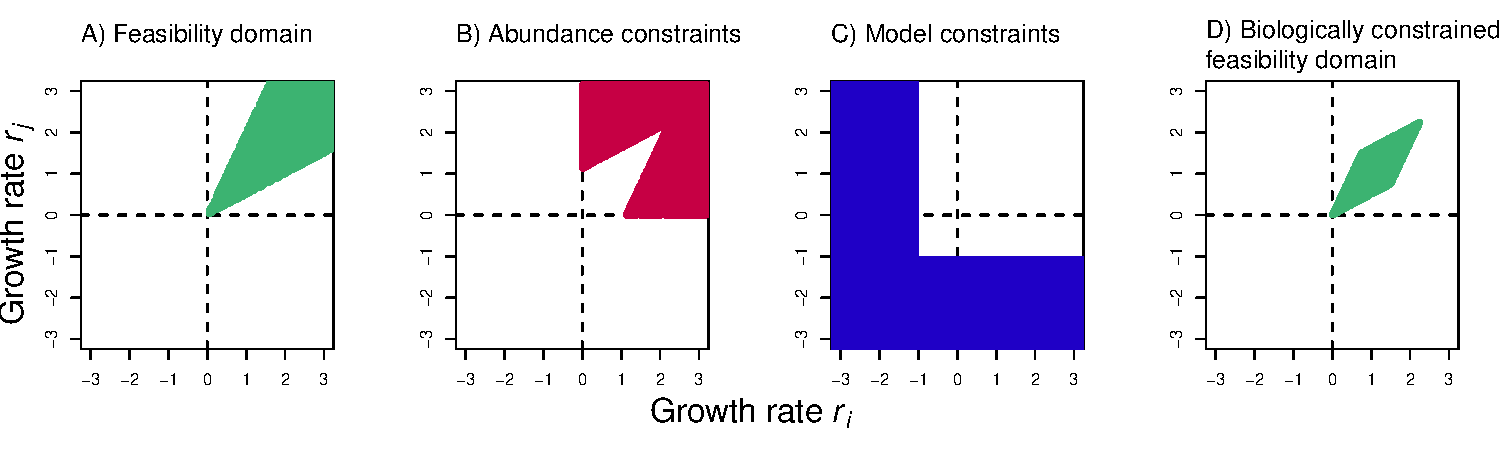
\includegraphics[width=1\textwidth]{figures/chapter3_fig1.pdf}}
  \caption[Estimation of the biologically-constrained feasibility domain]{Estimation of the biologically-constrained feasibility domain ($\beta$). A) We show the feasibility domain (green) given a hypothetical competition matrix with intraspecific competition coefficients equal to $1$ and interspecific competition coefficients equal to $0.5$. B) Part of the parameter space corresponds to species equilibrium abundances that are greater than specified abundance constraints (red). For simplicity, we used the same hypothetical abundance constraints for both species of $N^* \le 1.5$. C) Part of the the parameter space also falls outside model-based constraints (blue), assuming both species' density dependence is described by the Beverton--Holt model. D) The space of the feasibility domain that does not overlap with abundance or model-based constraints gives the biologically-constrained feasibility domain ($\beta$, green). }
  \label{fig:domain}
\end{figure}


\subsubsection*{Distance from the edge}

If two species' set of growth rates $r_{i}$ and $r_{j}$ are inside $\beta$, the two species are predicted to coexist. But there is more information contained in this comparison than a yes or no outcome. For example, the further those growth rates are from the edge of $\beta$, the less likely it is that perturbations to them will change the coexistence prediction. The minimum distance from the set of growth rates to the edge of $\beta$ is a measure of the susceptibility of qualitative coexistence predictions to perturbations of species' growth rates and interactions. We called this minimum distance $\delta$. To indicate when species growth rates are outside $\beta$, we multiplied $\delta$ by negative one. Large, positive values of $\delta$  thus imply species are confidently coexisting, large negative values imply species are confidently excluding each other, and values closer to zero imply small perturbations might change the predicted outcomes. We describe how exactly we quantify $\delta$ in \autoref{appendix_B}


\subsubsection*{Relative coexistence ratio}

As a basis of comparison, it is also convenient to quantify the parameter space that allows both species to grow in monoculture. Importantly, this parameter space can also be expressed as an area, and this area is also subject to abundance and model constraints. We called this area $\gamma$, and mathematical details of how to calculate the size of it can be found in \autoref{appendix_B}. By comparing the size of the parameter space where both species can coexist ($\beta$) to the size of the space where species can grow in monoculture ($\gamma$), we can quantify the importance of interspecific interactions relative to intraspecific interactions. This comparison can be expressed as a ratio $\rho$ that we call the relative coexistence ratio. If this ratio is equal to one, then species coexistence is as likely as species growing in monoculture; if this ratio is lower than one, then the parameter space where the two species can coexist is smaller than the parameter space where each species can grow in monoculture,  and it is less likely they can coexist when interacting; finally, ratios bigger than one imply that species facilitate each other, and it is more likely for them to coexist when interacting than to grow in monoculture. We show an example of how different values of $\beta$ and $\gamma$ determine the values of $\rho$, as well as their relationship to the distance from the edge $\delta$ in Fig.~\ref{fig:rho_delta}.

\subsubsection*{An alternative model of density dependence}

%\subsection*{Alternative models for density dependence}

The Beverton--Holt model is only one of many phenomenological models used to describe density-dependent performance of annual plants. There is no general rule on how to choose the appropriate phenomenological model to describe the effect of species interactions, and it is often a choice governed by mathematical convenience \citep{mayfield2017higher}, the type of study system \citep{godwin2020empiricist}, and the governing paradigm around species interactions \citep{martyn2021identifying}. Indeed, there exists a plethora of related mathematical expressions that can quantify interactions between plants. One of them is the Ricker  model:
 \begin{equation}
 \label{Ricker}
   F_{i,t} = \lambda_{i} e^{(- \alpha_{ii}g_{i}N_{i,t} - \alpha_{ij}g_{j}N_{j,t})}\,,
\end{equation}
where the interpretation of the parameters remains the same as previously described \citep{ricker1954effects}. The Ricker model is known to be a biologically plausible and versatile model to quantify density dependence in annual plant communities, plus it has the virtue of being better able to capture both competitive and facilitative interactions \citep{mayfield2017higher,bimler_accurate_2018}.


\begin{figure}[H]
  \centerline{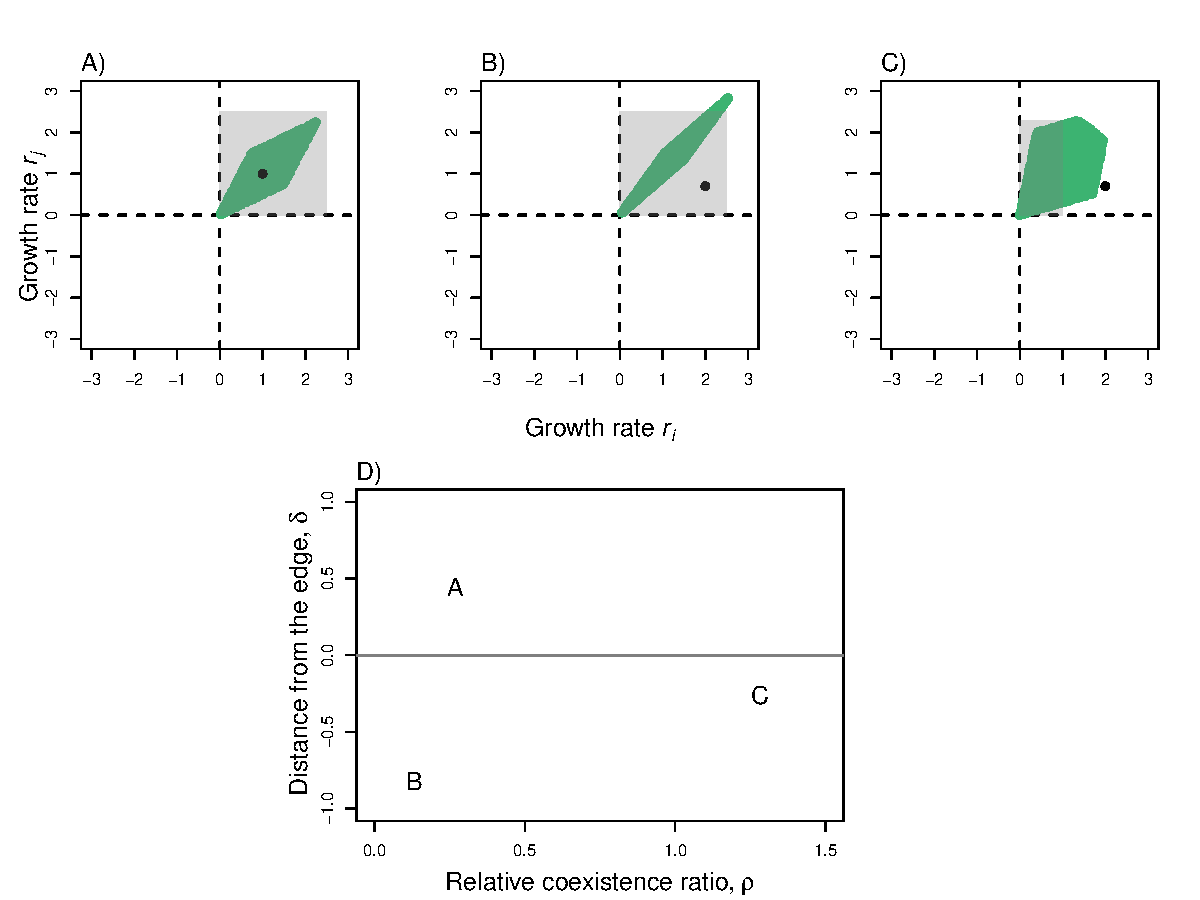
\includegraphics[width=1.1\textwidth]{figures/chapter3_fig2.pdf}}
  \caption[Examples of how different values of the biologically--constrained feasibility domain ($\beta$), the area in monoculture ($\gamma$), and species growth rates ($r_i$ and $r_j$) determine the values of the relative coexistence ratio ($\rho$) and the minimum distance from the edge ($\delta$).]{Examples of how different values of the biologically--constrained feasibility domain ($\beta$), the area in monoculture ($\gamma$), and species growth rates ($r_i$ and $r_j$) determine the values of the relative coexistence ratio ($\rho$) and the minimum distance from the edge ($\delta$). In A), B), and C) we show three hypothetical combinations of the biologically-constrained feasibility domain ($\beta$ in green), the parameter space where species can grow in monoculture ($\gamma$ in light grey), and a set of species growth rates (black circles). D) We show how the examples shown in A, B, and C correspond to different values of the relative coexistence ratio ($\rho$) and the distance from the edge ($\delta$).  }
  \label{fig:rho_delta}
\end{figure}


Similar to the process we followed from Eqns.~\ref{bh_equilibrium} to ~\ref{abundances}, the Ricker model has its own expression of growth rate at equilibrium. For species $i$, it is given by:
%\begin{equation}
%  r_{i} = 1 - \left(\frac{1-(1-g_{i})s_{i}}{g_{i}\lambda_{i}} \right).
%\end{equation}
%This expression necessarily implies that the model constraints on growth rates are different when using the Lotka--Volterra model than when using  the Beverton-Holt model: it has no lower limit but has an upper limit at one.
%In contrast, the composite growth rate for species $i$ in a Ricker model (Eqn.~\ref{Ricker}) is:
\begin{equation}
  r_{i}=\ln\left(\frac{g_{i}\lambda_{i}}{1-(1-g_{i})s_{i}}\right).
\end{equation}
This expression necessarily implies that the model constraints on growth rates are different when using the Ricker model than when using  the Beverton--Holt model: it has no model-based constraints on the lower and upper bounds of species growth rates. We summarize each of the models presented so far, their expressions of growth rates at equilibrium, and their lower and upper bounds in Table \ref{tab:definitions}


\begin{table}[h]

  \fontsize{10}{10}\selectfont
  \caption[Equilibrium growth rates and model constraints for the two models we used used to make coexistence predictions]{Equilibrium growth rates and model constraints for the two models we used used to make coexistence predictions. Growth rates are given by solving each model's equilibrium conditions in terms of seed densities. Upper and lower bounds are the result of how parameter bounds impact the values growth rate can take given the phenomenological model used to quantify density dependence.}
  \centering
  \label{tab:definitions}
 \begin{tabular*}{1\textwidth}{l @{\extracolsep{\fill}}lllll}
  \toprule
Model     & Growth rate & Lower bound& Upper bound \\\midrule
Beverton--Holt  &    $-1 + \left( \frac{g_{i}\lambda_{i}}{1-(1-g_{i})s_{i}} \right)$&  -1 &   Inf \\

%Lotka-Volterra  & $1 - \left(\frac{1-(1-g_{i})s_{i}}{g_{i}\lambda_{i}} \right)$          & -Inf &  1 \\
Ricker    & $\ln\left(\frac{g_{i}\lambda{i}}{1-(1-g_{i})s_{i}}\right)$  &   -Inf       &  Inf\\
\bottomrule
\end{tabular*}
\end{table}

\subsubsection*{Multi-model predictions of species coexistence}

By parameterizing a phenomenological model of plant competition, like the Beverton--Holt (Eqn.~\ref{Beverton-Holt}), we get a description of how seed set decreases with neighbor density. Perhaps more importantly, by linking this model to  Eqn.~\ref{annual_plant} we can make a prediction about whether or not two species are able to coexist. So far, we have been working with the implicit assumption that the same model describes the density dependence of the two species. However, there is no \textit{a priori} reason to assume this is the case, especially in an empirical case where different models can provide comparable fits \citep{hart2018quantify}.


To predict coexistence using a different density-dependence model per species, we still must solve for species equilibrium abundances as a function of growth rates and competition (Eqn.~\ref{abundances}). Unlike the single-model approach, each species' growth rate has its own formulation based on the model describing each species realized fecundity (Table \ref{tab:definitions}). As in the previous approach, if Eqn.~\ref{abundances} predicts positive abundances for both species within the bounds of each species' model and abundance constraints, species are predicted to coexist. Importantly, both $\beta$ and $\gamma$ become a function of four potential constraints: the set of lower and upper bounds per species. Having imposed those constraints, the relative coexistence ratio $\rho$ and the distance from the edge $\delta$ can again be calculated as described previously.


\subsection*{The interplay of different forms of uncertainty}

\subsubsection*{Data}

To assess the empirical relevance of different sources of uncertainty, we made coexistence predictions using parameter estimates inferred directly from a set of competition experiments. During 2017, we conducted pairwise competition experiments between two annual plants, \textit{Vellia rosea} and \textit{Trachymene cyanopetala}. Our experiments took place in the West Perenjori Nature Reserve in Western Australia (-29.479$^{\circ}$S, 116.199$^{\circ}$E). The reserve is dominated by York gum-jam woodlands, which support an understory of mixed native and exotic annual grasses and forbs \citep{dwyer2015climate}.

Using locally-collected seeds, we set up pairwise response--surface experiments. Response--surface experiments vary the densities of both species independently by using treatments with factorial combinations of the two species at two or more densities, and have the advantage of being able to accurately distinguish intra and interspecific competition \citep{inouye_response_2001, hart2018quantify}. To study how abiotic conditions change coexistence predictions, we conducted the experiments in two contrasting environments: a \textit{woody} environment, where plants interacted within 30 cm of woody debris, and a \textit{open} environment, where plants interacted at least 1 m outside the woody debris.

To implement our response--surface experiments, in October 2017 we first weeded out aboveground biomass of plants inside of circular plots with a 7.5 cm radius. This neighborhood radius is sufficiently large to capture local plant--plant interactions within the study system \citep{martyn2021identifying}. Each plot was then sown at different densities of each species as a focal: an invasion density where only one individual was sown, low density (15 seeds in total), medium density (30 seeds in total), and high density (60 seeds in total). In each plot, we also varied the densities with which the non-focal species was sown: either absent, medium or high. Treatments therefore consisted of combinations of the density of each species sown as a focal, the density of each species sown as a competitor, and the environment where interactions took place. We had four replicates per treatment, which yielded 256 plots in total. Plants germinated, and we thinned plots in composition in July 2018 (i.e., we weeded out neighbors that were not originally sowed). We collected the seeds produced after the growing season in October 2018 and also counted the number of conspecifics plant individuals ($n_{i}$), heterospecifics ($n_{j}$), and other neighbors ( $n_{k}$ i.e., plants that germinated after the plots were thinned in composition) in the plot at the time of seed collection.

Finally, we relied on a different set of data to obtain estimates of the survival and germination rates of each of our focal species in the field \citep{towers2021variable}, as well as the maximum abundance each species could achieve in the neighborhood radius where interactions took place. We show these values of seed survival rate, germination rate, and maximum abundance per species in \autoref{appendix_B}.

\subsubsection*{Statistical inference}

We fit Eqns.~\ref{Beverton-Holt} and~\ref{Ricker} separately for both of our focal species in order to get the relevant parameter estimates necessary to make coexistence predictions. For both species, we fit these non-linear models with a Bayesian framework using Hamiltonian Monte Carlo (HMC) methods. We used Bayesian inference to explicitly incorporate the uncertainty surrounding model parameters in probability distributions \citep{mcelreath_statistical_2018}. Across all models, we explicitly accounted for the environment where seeds were sown in our parameter estimates. For all of the parameters across all models, we did this by allowing the \textit{woody} environment to act as a dummy variable, $W$, that indicates the change in the environmental condition. For example, the fecundity in the absence of competition for species $i$ while in the \textit{woody} environment would be given by $\lambda_{i} + \lambda_{i,w}W$, where parameters with the subscript $w$ quantify the change due to the \textit{woody} environment.


For all models and all environmental conditions, we constrained the fecundity in the absence of competition  to be positive in order to keep our predictions biologically plausible. However, we did not constrain interaction parameters to be positive, allowing them to capture both competitive and facilitative interactions. Across all model fits, we included an extra term ($\alpha_{ik}$) to account for the effect of unidentified species in the experiment ($n_{k}$). We fit this extra interaction term to improve the parameter estimates  related to our focal species, but because we do not know their other parameters we could not model coexistence outcomes with these other neighbors.

We assumed the response variable, seeds produced per focal individual, followed a Poisson distribution for both species. Consequently we fit our non-linear models using the Poisson family and the identity link. We used the same weakly informative priors for the parameters in the Beverton--Holt model (Eqn.~\ref{Beverton-Holt}) and the Ricker model (Eqn.~\ref{Ricker}). As an example, the full description of the Beverton--Holt model for species $i$ is:

\begin{align}
 F_{i} \sim& {\textrm{Poisson}}(\rho_{i}) && \\
\rho_{i} =& \frac{e^{\lambda_{i} + \lambda_{i,w}W}} {1 + (\alpha_{ii} + \alpha_{ii,w}W)n_{i} + (\alpha_{ij} + \alpha_{ij,w}W) n_{j} + (\alpha_{ik} + \alpha_{ik,w}W)n_{k}} &&   \\
{ \left \{ \lambda_{i}, \lambda_{i,w} \right \}} \sim& {\textrm{Normal}}(0,1) &&\\
 { \left \{ \alpha_{ii}, \alpha_{ii,w} \right \}} \sim& {\textrm{Normal}}(0,1) &&\\
 {\left \{ \alpha_{ij}, \alpha_{ij,w} \right \}} \sim& {\textrm{Normal}}(0,1) &&\\
 {\left \{ \alpha_{ik}, \alpha_{ik,w} \right \}} \sim& {\textrm{Normal}}(0,1) &&
\end{align}

We fit all models using the function \textit{brm} from the package \textit{brms} \citep{burkner_advanced_2017} in the statistical program R version 4.0.2 \citep{Rcore}. For each model, we ran four chains with a warmup of 2000 iterations and 2000 sampling iterations. We determined convergence when trace plots were well mixed and stationary and when the Gelman--Rubin convergence diagnostic (Rhat) was less than 1.05 for all parameters \citep{vehtari_rank-normalization_2020}.

We compared the fits of each model for each species using the Leave-One-Out cross-validation Information Criteria (LOOIC). This goodness of fit measure is used for estimating the out-of-sample prediction accuracy of Bayesian models and provides a measure of model fit that is penalized for the number of model parameters. As with other information criteria, lower values of LOOIC correspond to better supported models. Additionally, LOOIC is more robust for models with weak priors or influential observations compared to other information criteria \citep{vehtari2017practical}. We calculated out-of-sample deviance separately for models in \textit{open} and \textit{woody} environments because LOOIC is calculated additively over observations. We also calculated Akaike weights for each model in each environmental condition, which can be interpreted as an estimate of the probability that the model will make the best predictions of new data, based on the set of models considered \citep{mcelreath_statistical_2018}

\subsubsection*{Predictions incorporating uncertainty}

To study how model formulation changes predictions of species coexistence, we used our framework to make predictions using median parameter estimates and a different model per species (Eqn.~\ref{Beverton-Holt} or ~\ref{Ricker}). We examined all the possible combinations of each species being defined by a different model, which yielded a total of 4 different predictions. Furthermore, we also explored how abiotic conditions change predicted coexistence outcomes by making predictions using median parameter estimates in the \textit{open} and \textit{woody} condition. We therefore had a total of 8 coexistence predictions (4 for each environmental condition), as well as the corresponding values of $\beta$, $\gamma$, $\rho$, and $\delta$.


To incorporate parameter uncertainty, we made predictions using 500 draws from the parameters' posterior distributions. For each of the 8 predictions made using median parameter values, this gives us 500 additional coexistence predictions. Posterior distributions of parameters contain the relative plausibility of different parameter values, conditional on the data and the model we used \citep{mcelreath_statistical_2018}. This approach yielded a posterior distribution of coexistence outcomes, as well as distributions of $\beta$, $\gamma$, $\rho$, and $\delta$ values.

For each model combination and each environmental condition, we determined the proportion of posterior predictions that predicted coexistence and competitive exclusion driven by \textit{Vellia rosea} or \textit{Trachymene cyanopetala}. We also calculated the combined LOOIC and weight for each model combination as the sum and product of both model’s LOOIC and weights, respectively. Finally, we  defined the weighted average of our coexistence predictions as the combined model weight in a given environmental condition, and the proportion of coexistence outcomes. Our approach thus allowed us to not only make predictions incorporating one source of uncertainty at a time but to integrate multiple sources of uncertainty together into a probabilistic interpretation of species coexistence.

\section*{Results}

Model comparison using LOOIC showed that the Beverton--Holt model was the preferred model for both species in both environments since it consistently had the lowest LOOIC score (Table \ref{tab:compare}). However, Akaike weights showed that the Ricker model shared some of probability to make the best prediction of new data for the species \textit{Vellia rosea} in both environments (Table \ref{tab:compare}). Indeed, some parameter values and their distributions overlap between the two models for both species (Figs.~ \ref{fig:vero_dist} and \ref{fig:trcy_dist} in \autoref{appendix_B}).


\begin{table}[H]
\centering
\fontsize{12}{10}\selectfont
\caption[Model comparison in the \emph{open} and \emph{woody} environments]{Model comparison in the \emph{open} and \emph{woody} environments. LOOIC (leave-one-out cross-validation information criteria) penalizes models for the number of parameters, and the lowest value reflects the best-performing model. The weight for each model is an estimate of the probability that the model will make the best predictions of new data based on the the set of models considered.}
\label{tab:compare}
\resizebox{1\textwidth}{!}{\begin{tabular}{lllrrrr}
  \hline
\multirow{2}{*}{Species} & \multirow{2}{*}{Model} & \multicolumn{2}{c}{Open} & \multicolumn{2}{c}{Woody} \\
       & & LOOIC & Weight & LOOIC & Weight \\
  \hline
\textit{Vellia rosea} & Beverton--Holt & 1001.16 & 0.99 & 1006.80 & 0.95 \\
%\textit{Vellia rosea} & Lotka-Volterra & 1050.97 & 0.00 & 1061.31 & 0.00  \\
\textit{Vellia rosea} & Ricker & 1017.99 & 0.01 & 1018.44 & 0.05 \\
\textit{Trachymene cyanopetala} & Beverton--Holt & 2025.51 & 1.00 & 2049.27 & 1.00 \\
%\textit{Trachymene cyanopetala} & Lotka-Volterra & 2267.05 & 0.00 & 2323.90 & 0.00 \\
\textit{Trachymene cyanopetala} & Ricker & 2048.80 & 0.00 & 2082.25 & 0.00 \\
   \hline
\end{tabular}}
\end{table}

\subsection*{Structural sensitivity in the \emph{open} environment}

In the \textit{open} environment, median predictions of species coexistence were contingent on the model formulation used for both species (triangles on Fig.~\ref{fig:open}). We predicted \textit{Vellia rosea} and \textit{Trachymene cyanopetala} would coexist in three of the model combinations we explored, while we predicted competitive exclusion of \textit{Vellia rosea} when the predictions used the Ricker model for \textit{Vellia rosea} and the Beverton--Holt model for \textit{Trachymene cyanopetala} (Fig.~\ref{fig:open}) .

We predicted the median relative coexistence ratio ($\rho$) would be around 0.5 for all of the model combinations examined, implying that interspecific interactions were competitive and approximately half the magnitude of intraspecific interactions (Fig.~\ref{fig:open}). On the other hand, the distance from the edge ($\delta$) was close to zero for three of the model combinations we explored (Fig.~\ref{fig:open}). That is, in the \textit{open} environment, median predictions of species coexistence---whether they predicted coexistence or competitive exclusion---were likely susceptible to change given small perturbations to either species growth rates or interaction coefficients.



\subsection*{Structural sensitivity \& environmental context dependency }


The consequences of structural sensitivity were different when interactions took place in the \textit{woody} environment. We predicted species coexistence in only one of the four model combinations we explored: when median predictions used the Beverton--Holt model for \textit{Vellia rosea} and the Ricker model for \textit{Trachymene cyanopetala} (Fig.~\ref{fig:woody}). That is, when we made predictions in the \textit{woody} environment, median parameter values mostly predicted competitive exclusion. However, unlike median predictions made for the \textit{open} environment, \textit{Trachymene cyanopetala} was predicted to be competitively excluded instead of \textit{Vellia rosea} (Fig.~\ref{fig:woody}). Additionally, our median estimates of $\rho$  were higher in the woody environment for 2 out of 4 model combinations examined (Fig.~\ref{fig:woody}). Note that $\rho$ values above one indicate that it is more likely for species to  coexist when growing together than when growing in monoculture.

In the \textit{woody} environment, estimates of $\delta$ were mostly negative (Fig.~\ref{fig:woody}). That is, for most of the model combinations we examined, species growth rates were far away from the biologically-constrained feasibility domain, and the coexistence outcome unlikely to change given small perturbations. These values of $\delta$ seem to be driving the changes in coexistence outcomes regardless of the values of $\rho$. Similar to the \textit{open} environment, the value of $\delta$ was positive and close to zero in the one instance where we predicted species coexistence.

\begin{figure}[H]
  \centerline{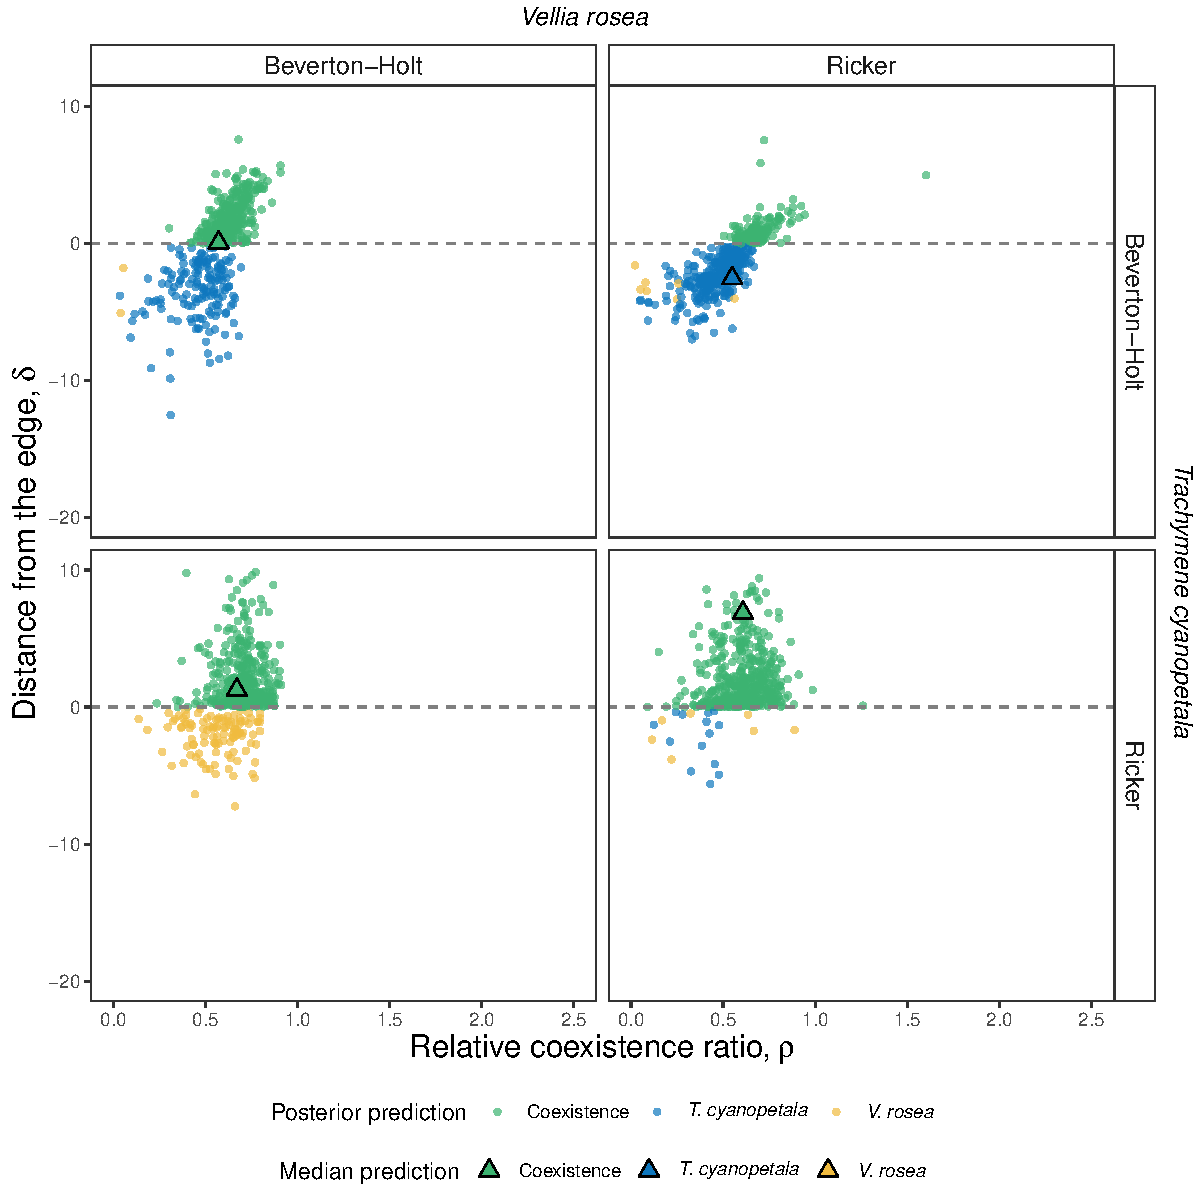
\includegraphics[width=1\textwidth]{figures/chapter3_fig3}}
  \caption[Predictions made with different model combinations in the \textit{open} environment]{Predictions made with different model combinations in the \textit{open} environment. Each panel corresponds to a different model combination, labels on the top indicate the model used for the species \textit{Vellia rosea}, and labels on the right show  the model used for \textit{Trachymene cyanopetala}.  In each panel, we show median estimates of $\rho$ and $\delta$ (triangles), and the color of these estimates indicates coexistence (green), competitive exclusion by \textit{Vellia rosea} (yellow), and competitive exclusion by \textit{Trachymene cyanopetala} (blue). Finally, we show the 500 predictions made using posterior draws of parameter values (circles) with the same color scheme.  }
  \label{fig:open}
\end{figure}

\begin{figure}[H]
  \centerline{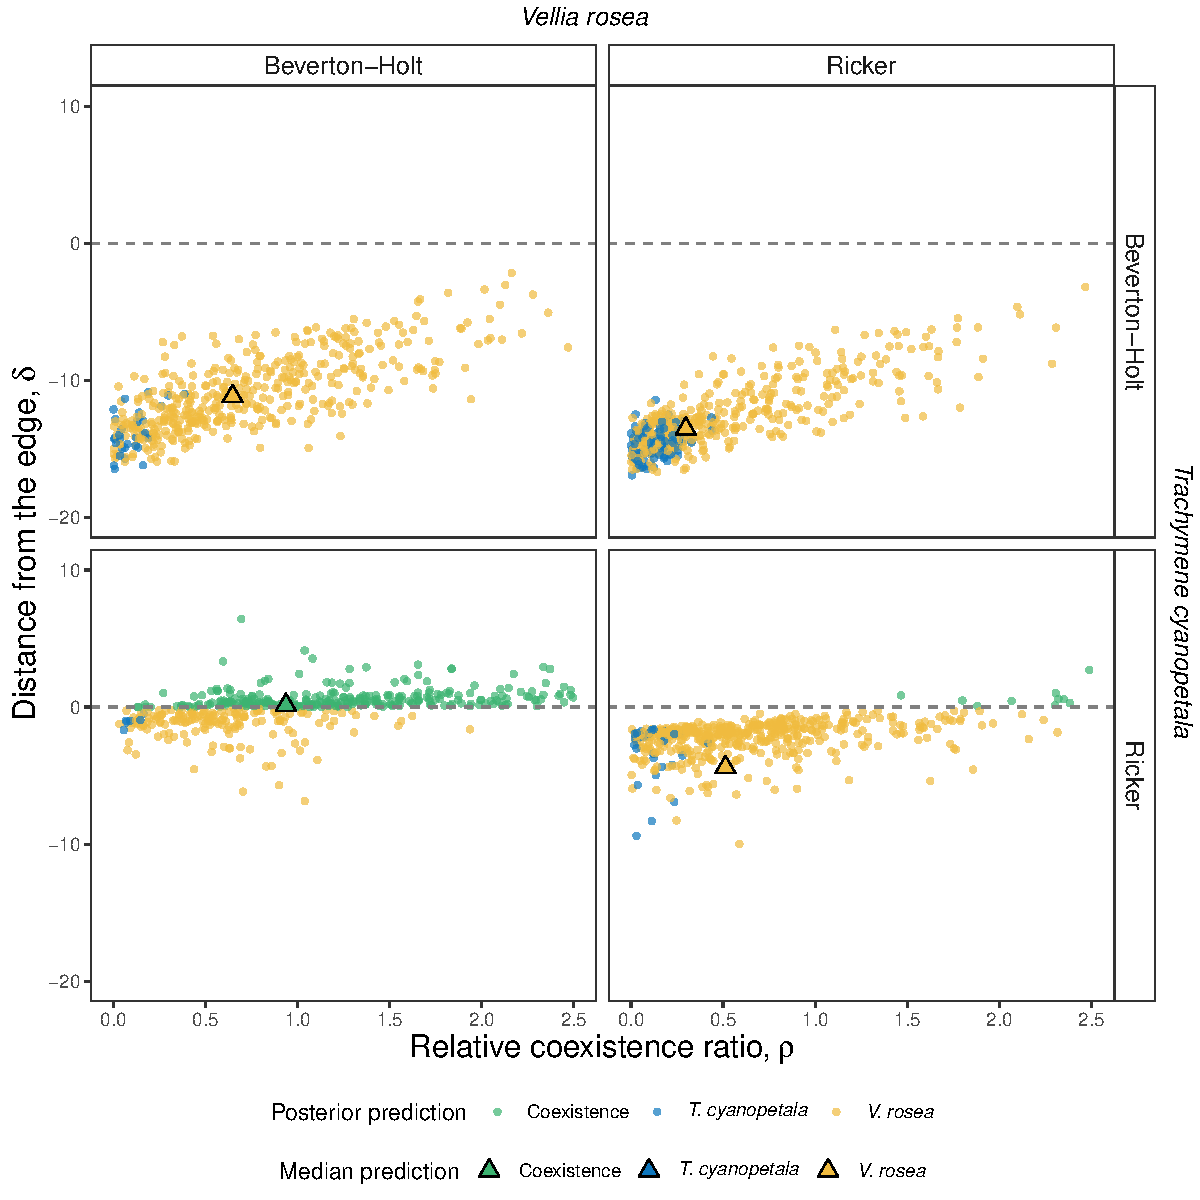
\includegraphics[width=1\textwidth]{figures/chapter3_fig4}}
  \caption[Predictions made with different model combinations in the \textit{woody} environment]{Predictions made with different model combinations in the \textit{woody} environment. Each panel corresponds to a different model combination, labels on the top indicate the model used for the species \textit{Vellia rosea}, and labels on the right show  the model used for \textit{Trachymene cyanopetala}.  In each panel, we show median estimates of $\rho$ and $\delta$ (triangles), and the color of these estimates indicates coexistence (green), competitive exclusion by \textit{Vellia rosea} (yellow), and competitive exclusion by \textit{Trachymene cyanopetala} (blue). Finally, we show the 500 predictions made using posterior draws of parameter values (circles) with the same color scheme.}
    \label{fig:woody}
\end{figure}

\subsection*{ Structural sensitivity, environmental context dependency \& parameter sensitivity }

Predictions made with the posterior distribution of parameter values could be quantitatively and qualitatively very different to predictions made with median parameter values (Figs.~\ref{fig:open} and \ref{fig:woody}). Importantly, the extent of parameter sensitivity depended on the models used and the environment where interactions took place. When species were interacting in the \textit{open} environment, we predicted both competitive exclusion and coexistence regardless of the outcome of the median prediction (Fig.~\ref{fig:open}). For posterior predictions of competitive exclusion, the species predicted to competitively exclude the other varied between model combinations and posterior draws (Fig.~\ref{fig:open}). The proportion of posterior draws that predicted coexistence ranged from 96\% to 33\%, depending on the model combination used to make predictions (Table~\ref{tab:proportions_open}).


In contrast, when interactions took place in the \textit{woody} environment  most of the posterior predictions resulted in competitive exclusion (Fig.~\ref{fig:woody}). For 3 out of 4 model combinations examined, the proportion of posterior draws that predicted coexistence was less than 10\% (Table~\ref{tab:proportions_woody}). However, the outcome of competitive exclusion varied  between  posterior predictions. That is, even if species were predicted to be confidently experiencing competitive exclusion, the outcome of competition was uncertain (Fig.~\ref{fig:woody}).


The probability of predicting species coexistence given each phenomenological model used and the proportion of posterior predictions of coexistence was 67\% in the \textit{open} environment when we used the Beverton--Holt model to describe the dynamics of both species (Table~\ref{tab:proportions_open}). Other model combinations had little statistical support  (Table~\ref{tab:proportions_open}). Similarly, in th \textit{woody} environment, the model combination where the Beverton--Holt model described the dynamics of both species had most of the statistical support (Table~\ref{tab:proportions_woody}). However, that model combination also confidently predicted competitive exclusion (Table~\ref{tab:proportions_woody}). Other model combinations in the \textit{woody} environment varied in their extent of posterior draws that predicted coexistence, however, they also had little statistical support (Table~\ref{tab:proportions_woody}).


\begin{table}[H]
%\begin{table}[]
\caption[Combined LOOIC, weights and proportion of coexistence for different model combinations in the \textit{open} environment]{Combined LOOIC, weights and proportion of coexistence for different model combinations in the \textit{open} environment. Combined LOOIC and weights were calculated as the sum and product of both model's LOOIC and weights, respectively. Proportion of coexistence quantifies the proportion of coexistence predictions relative to competitive exclusion predictions for each model combination.}
\label{tab:proportions_open}
\resizebox{1\textwidth}{!}{\begin{tabular}{@{}llllllll@{}}
\toprule
\textit{V. rosea}   & \textit{T. cyanopetala} &  Combined  & Combined  & Proportion & Proportion & Proportion                                                          \\
model          & model        &  LOOIC        & weight &   \textit{V. rosea} wins &  \textit{T. cyanopetala} wins & of coexistence      \\
\midrule
Beverton--Holt & Beverton--Holt         & 3026.66       & 0.99            & 0.01 & 0.31 &  0.68           \\
Ricker         & Beverton--Holt         & 3043.50       & 0.01            & 0.02 & 0.66& 0.33            \\
Beverton--Holt & Ricker                 & 3049.96       & 0.00            & 0.22 & 0.00 & 0.78                \\
Ricker         & Ricker                 & 3066.79       & 0.00            & 0.01 & 0.03 & 0.96            \\ \bottomrule
\end{tabular}}
%\end{table}
\end{table}

\vspace{10mm}

% DBS: Need to add columns below for competitive exclusion of each species

\begin{table}[H]
%\begin{table}[]
\caption[Combined LOOIC, weights and proportion of coexistence for different model combinations in the \textit{woody} environment]{Combined LOOIC, weights and proportion of coexistence for different model combinations in the \textit{woody} environment. Combined LOOIC and weights were calculated as the sum and product of both model's LOOIC and weights, respectively. Proportion of coexistence quantifies the proportion of coexistence predictions relative to competitive exclusion predictions for each model combination.}
\label{tab:proportions_woody}
\resizebox{1\textwidth}{!}{\begin{tabular}{@{}llllllll@{}}
\toprule
\textit{V. rosea}   & \textit{T. cyanopetala} &  Combined  & Combined  & Proportion      & Proportion & Proportion                                                      \\
model          & model        &  LOOIC        & weight  &   \textit{V. rosea} wins &  \textit{T. cyanopetala} wins & of coexistence               \\
\midrule
Beverton--Holt & Beverton--Holt         & 3056.07       & 0.95           & 0.93 & 0.06 & 0.01          \\
Ricker         & Beverton--Holt         & 367.71       & 0.05           & 0.78 & 0.22 & 0.00           \\
Beverton--Holt & Ricker                 & 3089.05       & 0.00            & 0.34 & 0.01 & 0.65                \\
Ricker         & Ricker                 & 3100.69       & 0.00            &0.88 & 0.07 & 0.05            \\ \bottomrule
\end{tabular}}
%\end{table}
\end{table}



\subsection*{ The drivers of parameter sensitivity }

To better understand parameter sensitivity, we made predictions of $\beta$, $\gamma$ $\rho$, and $\delta$ holding all parameters but one at their median
estimate and for the other we used draws from its posterior distribution (Fig.~\ref{fig:params}). Since it was consistently the best fit model, we used the Beverton--Holt model for both species. We found that parameter sensitivity was driven mostly by a few key parameters. In both environments, predictions that substantially deviated from the median prediction were mainly driven by uncertainty surrounding the competitive effects of \textit{Trachymene cyanopetala} (Fig.~\ref{fig:params}).


\begin{figure}[H]
  \centerline{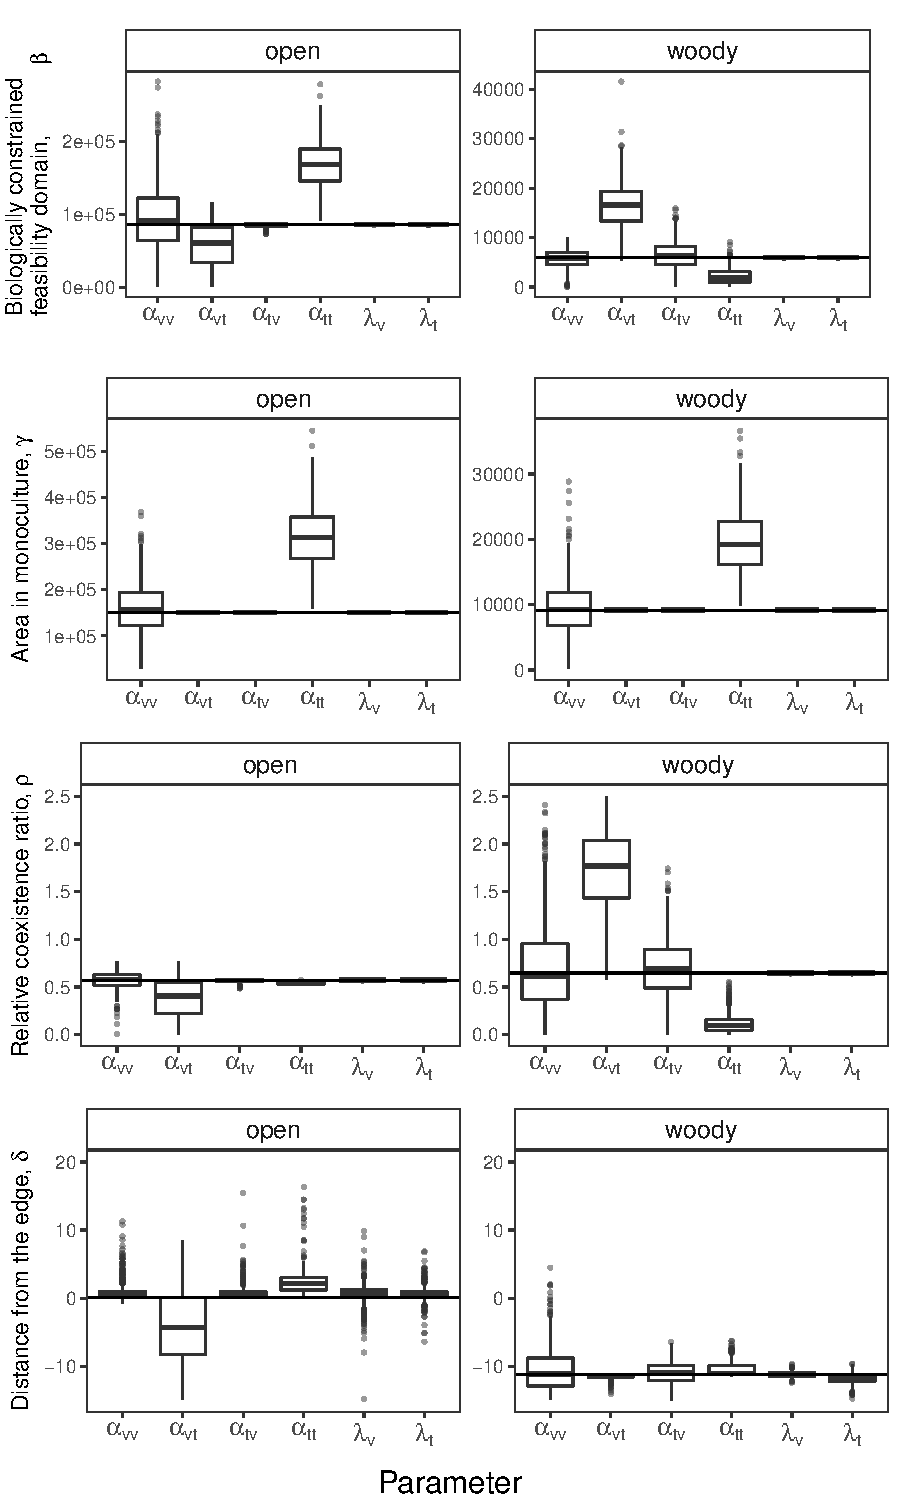
\includegraphics[width=.95\textwidth]{figures/chapter3_fig5.pdf}}
  \caption[Predictions of $\beta$, $\gamma$, $\rho$, and $\delta$  made while including the posterior distribution of each parameter separately and using the Beverton--Holt model for both species in both environments]{Predictions of $\beta$, $\gamma$, $\rho$, and $\delta$  made while including the posterior distribution of each parameter separately and using the Beverton--Holt model for both species in both environments. The parameter names on the x-axis denote the parameter whose distribution was sampled from. The subscript $v$ in parameter names denotes the species \textit{Vellia rosea}, while the subscript $t$ denotes the species \textit{Trachymene cyanopetala}. The solid black line in each panel denotes predictions when all parameters are set to their median estimates. Each boxplot extends from the first to third quantiles of the corresponding posterior predictions and the line inside the box indicates the median posterior prediction.   }
    \label{fig:params}
\end{figure}

\section*{Discussion}

Our results show that using phenomenological models to predict whether or not a pair of species can coexist is far from a trivial matter. Indeed, even seemingly subtle differences led to predictions of both coexistence and competitive exclusion based around the exact same experimental data. Even in the cases where we predicted competitive exclusion, the predicted dominant species varied between predictions. Nonetheless, our analyses also showed that the uncertainty surrounding our predictions can be dismantled and understood by understanding  differenes between models, the environment where models were parameterized, and the uncertainty associated to certain parameter values.

%: the difference between predictions can be explained based on models used to describe the interactions between species and the environment where models were parameterized. Incorporating parameter sensitivity further enriched our understanding of species coexistence as it showed the confidence of our specific predictions that species were likely able to coexist or not which, combined with model weights, allowed us to quantify the holistic probability of predicting species coexistence.


In our experimental system, the Beverton--Holt model was the best phenomenological description of how seed set changed with neighbor density, for both species in both environments (Table \ref{tab:compare}). The Beverton--Holt model frequently provides a good phenomenological fit for annual plant data
\citep{levine2009importance, godoy_phenology_2014, godoy_phylogenetic_2014}. However, the Ricker model shared some of the model weight with the Beverton--Holt model for \textit{Vellia rosea} in our experimental system, in both environmental conditions (Table \ref{tab:compare}). It is often the case in annual-plant studies that more than one phenomenological model has statistical support for different species or sites \citep{levine2009importance,mayfield2017higher,bimler_accurate_2018,martyn2021identifying}. Nonetheless, exploring predictions made by more than one model is not common practice in the study of species coexistence, unlike the study of other ecological processes like predator--prey dynamics \citep{myerscough1996stability,fussmann2005community,aldebert2018community}. By limiting our predictions to a single type of phenomenological model, we not only have to ignore other models that share statistical support, but we also limit our understanding of how model formulation itself changes our predictions.

%\vspace{5mm}
%\noindent\textbf{Structural Sensitivity}

\subsection*{Small differences, amplified}

We showed that predictions of species coexistence using the annual-plant model are structurally sensitive. Focusing on the \textit{open} environment, median estimates of $\rho$ and $\delta$  were similar in all of the model combinations we explored; coexistence outcomes were not (Fig.~\ref{fig:open}). Our study thus provides another clear example where predictions made with different models can be quantitatively similar and still have different qualitative properties, one of the hallmarks of structural sensitivity \citep{flora_structural_2011}.  Structural sensitivity can arise because slight perturbations in model formulation become largely amplified \citep{flora_structural_2011, wood1999super}, and predictions can be structurally sensitive in different ways depending on the qualitative behavior examined \citep{flora_structural_2011, aldebert2018community}. In the case of coexistence outcomes, predictions require the choice of a model to use for each species, which can further amplify small differences between models.

In the \textit{open} environment, we predicted coexistence in 3 out of 4 model combinations we explored (Fig.~\ref{fig:open}). Overall, the Beverton--Holt and the Ricker model predicted intraspecific interactions to be larger than interspecific interactions for both species (Figs.~S1 and S2), which tends to promote coexistence since species limit themselves more than what they limit others \citep{chesson_general_2000}. We only predicted competitive exclusion when we used the Ricker model for \textit{Vellia rosea} and the Beverton--Holt model for \textit{Trachymene cyanopetala} (Fig.~\ref{fig:open}). The differences between intraspecific and interspecific interactions for \textit{Vellia rosea} predicted by the Ricker model were slightly smaller than the ones predicted by the Beverton--Holt model (Fig.~\ref{fig:vero_dist} in \autoref{appendix_B}). Furthermore, the fecundity in the absence of competition of \textit{Trachymene cyanopetala} was predicted to be higher by Beverton--Holt model than by the Ricker model (Fig.~\ref{fig:trcy_dist} in \autoref{appendix_B}). These two small differences between models together resulted in a more restricted feasibility domain, and a shift in the position of species growth rates in the parameter space, compared to other model combinations. These changes caused the growth rates to fall outside $\beta$, $\delta$ to have a negative sign, and to predict the competitive exclusion of \textit{Vellia rosea} (Fig.~\ref{fig:open}).

% DBS: I like the text in the following paragraph, but what is it doing here? It reads like an intro, an abstract, or a conclusion. I think it needs to get cut...
%Species coexistence is determined by multi-level processes acting simultaneously, and studying it often involves a process of abstraction from the reality to mathematical objects such as phenomenological models \citep{levins_strategies_2006}. This process of abstraction makes it difficult to disentangle exactly why some model combinations give different results than the rest. Structural sensitivity is likely to arise when multi-level processes are summarized into equations after adopting assumptions regarding the complexity of the biological system \citep{aldebert2018community}. Thus, predictions of species coexistence are particularly likely to show structural sensitivity.

\subsection*{The importance of environmental context}

The extent of structural sensitivity observed in our focal system changed in the \textit{woody} environment. When we made predictions using median parameter estimates in the  \textit{woody} environment, 3 out of 4 model combinations  predicted competitive exclusion (Fig.~\ref{fig:woody}). The increased likelihood of predicting competitive exclusion compared to the \textit{open} environment seemed to be driven by several factors. One of them is that predicted interspecific interactions were larger than intraspecific interactions for \textit{Vellia rosea} using both models (Fig.~\ref{fig:vero_dist} in \autoref{appendix_B}), which resulted in a smaller $\beta$ in the \textit{woody} environment. However, since all intraspecific interactions were predicted to be weaker in the \textit{woody} environment compared to the \textit{open} environment for all models (Figs.~\ref{fig:vero_dist} and \ref{fig:trcy_dist} in \autoref{appendix_B}), the predicted values of $\gamma$ also decreased. Thus, values of $\rho$ in the \textit{woody} environment were larger in two out of four cases (Fig.~\ref{fig:woody}).

Furthermore, both species were predicted to have lower fecundities in the absence of competition compared to the \textit{open} environment, which supports previous empirical studies that have recorded that plant abundances in this system decline while growing inside litter \citep{wainwright2017effects} (Figs.~\ref{fig:vero_dist} and \ref{fig:trcy_dist} in \autoref{appendix_B}). Of the two species, \textit{Trachymene cyanopetala} was predicted to experience a sharper reduction in seed set by both models (Fig.~\ref{fig:trcy_dist},\autoref{appendix_B}). Thus, in the \textit{woody} environment, reductions in $\beta$ and changes in the predicted fecundity in the absence of competition for \textit{Trachymene cyanopetala} resulted in predictions of competitive exclusion of \textit{Trachymene cyanopetala} in three out of four model combinations (Fig.~\ref{fig:woody}). Even though the presence of woody debris in semiarid systems can reduce solar radiation and ameliorate drought stress \citep{wainwright2017effects}, our results suggest that species are less likely to coexist in this environment due to an increase in strength of interspecific interactions for \textit{Vellia rosea}, and a sharp reduction in the seed set of \textit{Trachymene cyanopetala}.

Our results  provide another example where interaction strengths, and thus coexistence predictions change with environmental conditions, a result that has been empirically demonstrated before in this system \citep{mayfield2017higher,wainwright2017diverse,bimler_accurate_2018}. Other studies have documented that both species indeed change their fecundities while growing inside coarse woody debris, but spatial mechanisms of coexistence between these two species have not been found \citep{towers2020requirements}. Importantly, the extent of environmental context dependency in our experimental system is determined by the models used to quantify density dependence for both species. That is, the effect of abiotic conditions can be enhanced or diminished in predictions of species coexistence due to use of phenomenological models.


% However, the variation in interaction strengths inside and outside woody debris could promote coexistence via the spatial storage effect \citep{sears2007new}, allowing, for example \textit{Vellia rosea} to exploit its differential response to the environment and to persist in the system. Importantly, the extent of environmental context dependency in our experimental system is determined by the models used to quantify density dependence for both species. That is, the effect of abiotic conditions can be enhanced or diminished in predictions of species coexistence due to use of phenomenological models.


%\vspace{5mm}
%\noindent\textbf{Parameter sensitivity}
\subsection*{Parameter uncertainty and the probability of predicting species coexistence}


Using a Bayesian Approach to fit models to data also allowed us to have a better understanding of the parameter uncertainty associated with our predictions. Our results showed that estimating pairwise coexistence only using median estimates of parameter values might bypass instances where the uncertainty encompasses outcomes different to the median prediction (Fig.~\ref{fig:open} and \ref{fig:woody}). Other approaches have incorporated parameter uncertainty in coexistence predictions by propagating standard errors \citep{matias2018experimental} or bootstrapping observations \citep{garcia2020cxr}. However, these approaches were only incorporated to show the robustness of predictions rather than to examine the causes and effects of parameter uncertainty in predictions of species coexistence.

%the probability of coexistence
Our results also show that even when we predicted competitive exclusion, the species we predicted to be competitively excluded varied across posterior draws (Fig.~\ref{fig:open} and \ref{fig:woody}). Other studies that have incorporated posterior distribution of parameter values  in coexistence predictions have also encountered this uncertainty regarding the outcome of competition \citep{terry2021natural}. However, they also found that posterior predictions mostly agree with predictions using median parameter values (i.e., species were confidently coexisting or not) \citep{terry2021natural}. Our results did not show as clear differences, particularly in the \textit{open} environment where species were very close to the coexistence boundary (Fig.~\ref{fig:open}).

%The differences in confidence of coexistences predictions might be explained due to the framework we used. Modern coexistence theory, a commonly used framework to quantify species coexistence \citep{chesson_general_2000, barabas_chessons_2018, chesson_updates_2018}, uses coexistence metrics that depend simultaneously on growth rates and competition coefficients. This creates an interdependence in coexistence outcomes \citep{song_consequences_2019} which, combined with the interrelationships between parameters, can dramatically affect the confidence with which conclusions are drawn from experimental data \citep{terry2021natural}. In contrast, our study uses an structural approach, in which competition and growth rates have distinct contributions to predictions of species coexistence \citep{rohr_structural_2014,saavedra_structural_2017, song_guideline_2018}, thus reducing the effect of interdependence of parameter values.


Importantly, the effect parameter sensitivity on predictions of species coexistence has been mostly interpreted as statements of uncertainty in the underlying data, rather than implying a probabilistic outcome \citep{terry2021natural,matias2018experimental}. Our study goes beyond that interpretation by combining model weights and posterior predictions to calculate the probability of predicting coexistence given the phenomenological models used to quantify density dependence. Our results suggest that given the uncertainty associated with our predictions, coexistence between \textit{Vellia rosea} and \textit{Trachymene cyanopetala} is likely in the \textit{open} environment (Table~\ref{tab:proportions_open}) and virtually impossible in the \textit{woody} environment (Table~\ref{tab:proportions_woody}).


Finally, our results also suggest that parameter sensitivity is mostly driven by the uncertainty of the competitive effect of \textit{Trachymene cyanopetala} (Fig.~\ref{fig:params}). Indeed, the posterior distribution of parameter values in the Beverton--Holt model that best captured the effect of \textit{Trachymene cyanopetala}, encompass a larger range of values compared to other competition coefficients (Fig.~\ref{fig:trcy_dist} in \autoref{appendix_B}). More accurate predictions of coexistence can be achieved by improving the estimates of parameters associated to the competitive effect of this species, for example with a separate experiment designed exclusively to capture the effects of \textit{Trachymene cyanopetala}  on itself and on \textit{Vellia rosea}.


\subsection*{Conclusion}


Predictions of species coexistence constitute the building blocks for many ecological studies, such as community assembly \citep{hillerislambers2012rethinking,kraft2015community, grainger_applying_2019}, the evolution of competitive communities \citep{letten2021using, pastore2021evolution}, or the role of species richness in ecosystem functioning \citep{godoy2020excess}. Many of these studies rely on phenomenological models of plant competition as the basis of their predictions. Species coexistence is determined by multi-level processes acting simultaneously, and studying it often involves a process of abstraction from the reality to mathematical objects such as phenomenological models \citep{levins2006strategies}. Structural sensitivity is likely to arise when multi-level processes are summarized into equations after adopting assumptions regarding the complexity of the biological system \citep{aldebert2018community}, making predictions of species coexistence made with phenomenological models particularly vulnerable. Furthermore our study has shown that different phenomenological models can enhance or diminish the effect of environmenatl context-dependency and parameter sensitivity, and thus our predictions of species coexistence. Overall, our study demonstrates that the interplay between different sources of uncertainty should not be ignored when we make predictions based on phenomenological models of plant competition.


\printbibliography
\end{refsection}

\begin{refsection}
\chapter{Coexistence of alleles} % Main chapter title
\label{Coexistence_alleles}

This is your coexistence of alleles manauscript

\end{refsection}
 % Chapter 4 - empty template
\part{Discussion}
\begin{refsection}
\chapter{Conclusion} % Main chapter title
\label{Conclusion}
\begin{flushright}{\slshape
    Where is the rest of the world? \\
    That is the question we must always ask about any model: \\
    where is the rest of the world?
    } \\ \medskip
    --- \textcite{levins2006strategies}
\end{flushright}

\bigskip

In this thesis, I show how to incorporate biotic and abiotic complexity in models of biotic interactions to increase model realism. Furthermore, I provide direct evidence that many models used to describe biotic interactions are oversimplistic since they fail to capture dynamics accurately by \textit{a priori} ignoring biotic and biotic factors. Throughout this thesis, I also show that increasing realism in models of biotic interactions has important repercussions on our understanding and predictions about the maintenance of diversity at ecological and evolutionary scales.

\section*{Summary of results}
In \autoref{Bee_foraging} I found that the abundance of co-foragers can substantially change the number of visits pollinators make. These results imply that it is necessary to account for the density of species other than the focal pair to characterize plant-pollinator interactions accurately. However, results from this chapter also show that the environmental context pollinators experience mediates density-dependent responses to co-foraging species. Thus, abiotic drivers can modify the number of visits made by pollinators through both density-independent and density-dependent responses. These two types of responses can cause the same environmental context to have opposite effects on floral visits. Such is the case of high resource abundance in our foraging experiment. Additionally, in this chapter I show that pollinators do not respond equally to all co-foraging species. Therefore the effects of biotic and abiotic drivers depend on the identity of the interacting species. Results from this chapter clearly show that including these levels of complexity in a model of floral visits is justified, despite the increasing number of parameters necessary to parameterize it. Since floral visitation is a good predictor of the strength of plant-pollinator interactions my results demonstrate that failing to account for biotic and abiotic complexity 

\section*{General Implications}
\subsection*{Model realism}
\subsection*{Diversity maintenance}
Models of mutualistic interactions are generally used to understand the number of species that can be maintainted in a community.

\section*{Future Directions}

\printbibliography
\end{refsection}

%\cleardoublepage % Empty page before the start of the next part

%----------------------------------------------------------------------------------------
%	THESIS CONTENT - APPENDICES
%----------------------------------------------------------------------------------------

%\appendix

%\part{Appendix} % New part of the thesis for the appendix

%\include{Chapters/Chapter0A} % Appendix A
%\include{Chapters/Chapter0B} % Appendix B
%\include{Chapters/Chapter0C} % HP manuscript - to fix: clash with xcolor package :(
%----------------------------------------------------------------------------------------
%	POST-CONTENT THESIS PAGES
%----------------------------------------------------------------------------------------

%\cleardoublepage% Bibliography

\label{app:bibliography} % Reference the bibliography elsewhere with \autoref{app:bibliography}

%\manualmark % Work-around to have small caps also here in the headline
%\markboth{\spacedlowsmallcaps{\bibname}}{\spacedlowsmallcaps{\bibname}} % Work-around to have small caps also
%\phantomsection

%\addtocontents{toc}{\protect\vspace{\beforebibskip}} % Place the bibliography slightly below the rest of the document content in the table of contents
%\addcontentsline{toc}{chapter}{\tocEntry{\bibname}}

\addcontentsline{toc}{chapter}{Bibliography}
\chapter*{Bibliography}

%\begin{flushright}{\slshape
 %   Hypothesen sind Netze, nur der wird fangen, der auswirft} \\ \medskip
  %  --- \textcite{novalis_novalis_1837}
%\end{flushright}

%\printbibliography[
%heading=none
%]

% \label{app:bibliography} % Reference the bibliography elsewhere with \autoref{app:bibliography}
%
\manualmark
\markboth{\spacedlowsmallcaps{\bibname}}{\spacedlowsmallcaps{\bibname}} % Bibliography

%\cleardoublepage% Declaration
\pdfbookmark[0]{Declaration}{declaration} % Bookmark name visible in a PDF viewer

\chapter*{Declaration} % Declaration section text

\thispagestyle{empty}

\begin{figure}[!htbp]
    \centering
    \includegraphics[width=\textwidth]{Chapters/Co-authorship-Form---Doctoral_dbs.pdf}
\end{figure} % Declaration

\cleardoublepage% Colophon (a brief description of publication or production notes relevant to the edition)

\pagestyle{empty}

\hfill

\vfill

\pdfbookmark[0]{Colophon}{colophon}

\section*{Colophon}

This document was typeset using the typographical look-and-feel \texttt{classicthesis} developed by Andr\'e Miede. The style was inspired by Robert Bringhurst's seminal book on typography ``\emph{The Elements of Typographic Style}''. \texttt{classicthesis} is available for both \LaTeX\ and \mLyX: 

\begin{center}
\url{https://bitbucket.org/amiede/classicthesis/}
\end{center}

\bigskip

\noindent\finalVersionString % Colophon

%----------------------------------------------------------------------------------------

\end{document}
